\documentclass[10pt,conference,letterpaper]{IEEEtran}

\usepackage[utf8]{inputenc}
\usepackage[T1]{fontenc}
\usepackage{silence}\WarningsOff[latexfont]

\usepackage{amsmath}
\usepackage{amsfonts}
\usepackage{amssymb}

\usepackage{graphicx}
\graphicspath{images/}
\usepackage{cite}
\usepackage{url}
% \usepackage{subfig}
\usepackage{subcaption}
\usepackage{float}
\usepackage[ruled,vlined,linesnumbered]{algorithm2e}
\SetKwProg{Fn}{Event}{}{}
\SetKw{And}{and}
\usepackage[binary-units,per-mode=symbol]{siunitx}
\sisetup{list-final-separator = {, and },detect-weight=true, detect-family=true}
\usepackage{booktabs}
\usepackage{pifont}
\usepackage{microtype}
\usepackage{textcomp}
\usepackage[american]{babel}
\usepackage[capitalise]{cleveref}
\def\figname{\csname cref@figure@name\endcsname\xspace}
\def\tabname{\csname cref@table@name\endcsname\xspace}
\def\secname{\csname cref@section@name\endcsname\xspace}
\def\eqpname{\csname cref@equation@name@plural\endcsname\xspace}
\crefname{algorithm}{Listing}{Lists.}
\Crefname{algorithm}{Listing}{Listings}
\SetAlgorithmName{Listing}{Listing}{List of Listings}
\crefname{lstlisting}{listing}{listings}
\Crefname{lstlisting}{Listing}{Listings}
\usepackage{xspace}
\usepackage{hyphenat}
\usepackage[draft,inline,nomargin,index]{fixme}
\fxsetup{theme=color}
\usepackage{grffile}
\usepackage{xfrac}
\usepackage{multirow}
%\usepackage[para]{footmisc}
\usepackage[font={small}]{caption}

\usepackage{tikz}
\usetikzlibrary{calc,shapes,arrows,fit,positioning}

\usepackage{listings}
\lstset{
   language=sh,
   columns=fixed,
   breaklines=true,
   breakatwhitespace=true,
   prebreak=\textbackslash,
   basicstyle=\ttfamily\small,
   showstringspaces=false,
   upquote=true,
   keywordstyle=\ttfamily\small
}

\usepackage{color}
\definecolor{gray}{rgb}{0.4,0.4,0.4}
\definecolor{darkblue}{rgb}{0.0,0.0,0.6}
\definecolor{cyan}{rgb}{0.0,0.6,0.6}


\lstdefinelanguage{XML}
{
  morestring=[b]",
  morestring=[s]{>}{<},
  morecomment=[s]{<?}{?>},
  stringstyle=\color{black},
  identifierstyle=\color{darkblue},
  keywordstyle=\color{cyan},
  morekeywords={xmlns,version,type}% list your attributes here
}


% fix cleveref and breqn
\makeatletter
\let\cref@old@eq@setnumberOld\eq@setnumber
\def\eq@setnumber{%
\cref@old@eq@setnumberOld%
\cref@constructprefix{equation}{\cref@result}%
\protected@xdef\cref@currentlabel{%
[equation][\arabic{equation}][\cref@result]\p@equation\eq@number}}
\makeatother

% reduce verbatim font size
\usepackage{etoolbox}
\makeatletter
\patchcmd{\@verbatim}
  %%%{\verbatim@font} %% blow up TexMaker formatting ???!!! 
  {\verbatim@font\small}
  {}{}
\makeatother

\RequirePackage{xstring}
\RequirePackage{xparse}
\RequirePackage[index=true]{acro}
\NewDocumentCommand\acrodef{mO{#1}mG{}}{\DeclareAcronym{#1}{short={#2}, long={#3}, #4}}
\NewDocumentCommand\acused{m}{\acuse{#1}}


\acrodef{ADV}{advertisement}
\acrodef{AS}{Autonomous System}{short-plural=es}
\acrodef{BGP}{Border Gateway Protocol}
\acrodef{BIRD}{BGP Internet Routing Daemon}
\acrodef{DPC}{Destination Partial Centrality}
\acrodef{eBGP}{Exterior BGP}
\acrodef{ERP}{Exterior Routing Protocol}
\acrodef{IoF}{Internet on FIRE}
\acrodef{IP}{Internet Protocol}
\acrodef{MRAI}{Minimum Route Advertisement Interval}
\acrodef{NH}{Next Hop}
\acrodef{RFC}{Request For Comment} 
\acrodef{TCP}{Transmission Control Protocol}
\acrodef{FSM}{Finite State Machine}

\newcommand\useallac{
\acused{IP}
\acused{TCP}
\acused{RFC}
}

\useallac

\newcommand{\figwidthfour}{0.78}
\newcommand{\figwidth}{0.78}
\newcommand{\figvspace}{-1.5em}
\newcommand{\update}{\texttt{UPDATE}\xspace}
\newcommand{\nodeset}{\ensuremath{\mathcal{V}}\xspace}
\newcommand{\destinationset}{\ensuremath{\mathcal{C}}\xspace}
\newcommand{\edgeset}{\ensuremath{\mathcal{E}}\xspace}
\newcommand{\graph}{\ensuremath{\mathcal{G(\nodeset,\edgeset)}}\xspace}
\newcommand{\pathset}{\ensuremath{\mathcal{C}}\xspace}
\newcommand{\ascentg}{\ensuremath{\mathcal{G_{A}}\xspace}}
\newcommand{\ascentnodeset}{\ensuremath{\mathcal{V^{\ascentg}}}\xspace}
\newcommand{\ascentedgeset}{\ensuremath{\mathcal{E^{\ascentg}}}\xspace}
\newcommand{\ascentgraph}{\ensuremath{\mathcal{\ascentg(\ascentnodeset,\ascentedgeset)}}\xspace}
\newcommand{\dpc}{\ensuremath{\Delta}\xspace}
\newcommand{\tr}{\ensuremath{T_{R}}\xspace}

\newcommand{\tierg}{\ensuremath{\mathcal{G_{T}}\xspace}}
\newcommand{\tiernodeset}{\ensuremath{\mathcal{V^{\tierg}}}\xspace}
\newcommand{\tieredgeset}{\ensuremath{\mathcal{E^{\tierg}}}\xspace}
\newcommand{\tiergraph}{\ensuremath{\mathcal{\tierg(\tiernodeset,\tieredgeset)}}\xspace}
\newcommand{\descentg}{\ensuremath{\mathcal{G_{D}}\xspace}}
\newcommand{\descentnodeset}{\ensuremath{\mathcal{V^{\descentg}}}\xspace}
\newcommand{\descentedgeset}{\ensuremath{\mathcal{E^{\descentg}}}\xspace}
\newcommand{\descentgraph}{\ensuremath{\mathcal{\descentg(\descentnodeset,\descentedgeset)}}\xspace}

\IEEEoverridecommandlockouts

\begin{document}

\title{SumUp 23-10-2020}
\author{
	\IEEEauthorblockN{Mattia Milani\IEEEauthorrefmark{1}}
    \IEEEauthorblockA{\IEEEauthorrefmark{1}Dept. of Information Engineering and Computer Science, University of Trento, Italy}
    \texttt{mattia.milani@studenti.unitn.it}
}


\maketitle

\section{Experiments Presentation}
\label{sec:mainIdea}

The goal of this document is, to sum up, and describe the experiments done up to 
now.
All the experiments were done using the software in this repository and are
fully replicable.
How to run and analyze the experiments is out of the scope of this document.

The experiments are divided in two main categories:
\begin{itemize}
	\item \textit{\textbf{Single node evaluation}}, in this group of experiments
		the goal is to analyze a single node evolution in the network;
	\item \textit{\textbf{Network evaluation}}, in this group of experiments 
		the evaluation is done on the entirety of the network.
\end{itemize}

\section{Goals}
\label{sec:goals}

Like I specified in \Cref{sec:mainIdea} all the experiments are divided into two
categories that are distinguished by the size of the analysis.
The simulation environment could be the same but the difference is in the
analysis of the evolution.

In the first case, \textit{\textbf{Single node evaluation}}, the goal of the
analyzer is to study a specific node and highlight the evolution of it.
The output of the analysis could be the \ac{FSM} of the node and the signalling
plot.

The signalling of a node represents all the possible outputs of a node.
A single output signal represents in a single experiment the messages transmitted
by the node, the result will be a mix of advertisements and withdraws in
a string like "A1W1A4A6W6"
This ouptuts signals, for each bunch of experiments, are collected in a CSV file
with the appearance frequency of each output signal.

In the second case, \textit{\textbf{Network evaluation}}, we are looking for
network results, evaluating the entire set of nodes and links.
This is done by studying the number of messages transmitted and the convergence time.

Given $T_{tx}$ as the time of the first transmission and $T_{rx}$ as the time of the
\textbf{last} reception the convergence time, $CT$, is given by the delta of those
times: $CT = T_{rx} - T_{tx}$.
The convergence is reached when the network becomes silent again.

\section{Environments}
\label{sec:input}

Multiple environments have been used for the experiments.
The main differences and properties of those environments are described in this
section.

The first environment that I used is a \textit{Fabrikant} environment with
different \ac{MRAI} settings.
This name comes from the particular graph used, described in \Cref{sec:graph}.
The four types of \ac{MRAI} used are:
\begin{itemize}
	\item \textit{\textbf{Fixed 30s}}, \ac{MRAI} is fixed for each link to 30 seconds;
	\item \textit{\textbf{No MRAI}}, \ac{MRAI} is fixed for each link to 0.0 seconds;
	\item \textit{\textbf{Ascendent}}, \ac{MRAI} will be doubled at each leach ($1-2-4-8-...$);
	\item \textit{\textbf{Descendent}}, Reverse of the ascendent case, \ac{MRAI}
		will be divided by two at each leach.
\end{itemize}

The second environment used is a \textit{clique} one, the graph is described in \Cref{sec:graph},
all the parameters of the environment are described in \Cref{sec:envDesc}
In all the clique experiments \ac{MRAI} has been fixed in all the links.
For each value of \ac{MRAI} has been done $10$ different experiments and \ac{MRAI}
goes from $0$ in the first group of experiments to $60$ in the last group.
For a total of $610$ runs in this topology.

The last one used is an \textit{Internet Like} environment. 
The graph is described in \Cref{sec:graph}, all the parameters are described in
\Cref{sec:envDesc}.
The main goal of this environment was to emulate, roughly, a real environment.
The main difference between different experiments on this environment was the
type of \ac{MRAI} applyed:
\begin{itemize}
	\item \textit{\textbf{Random MRAI}}, for each link the \ac{MRAI} value will
		be chosen with a uniform distribution between $[0.0, MRAI_{limit}]$,
		the network must respect a defined $MRAI_{mean}$ value
	\item \textit{\textbf{Fixed MRAI}}, for each link the \ac{MRAI} will be 
		equal to $MRAI_{mean}$
	\item \textit{\textbf{DPC}}, for each link the \ac{MRAI} will be setted
		according to the centrality of the node, process described in \Cref{sec:dpc}
\end{itemize}
In this environment has been run multiple experiments for each \ac{MRAI} type.
For each experiment, a new graph would be computed, so in the \textit{Random MRAI},
for the same $MRAI_{mean}$ value could exists multiple different graphs.

\section{Input Graphs}
\label{sec:graph}

In total three different base graphs has been used to produce all the results
in this document.

\subsection{Fabrikant Graph}
\label{subsec:fabrikant_graph}
The Fabrikant graph replicate what is described in the first figure in \cite{fabrikant}.
for simplicity, an example is reported here in \Cref{fig:fabr_graph}

\begin{figure}[tb]
	\centering
	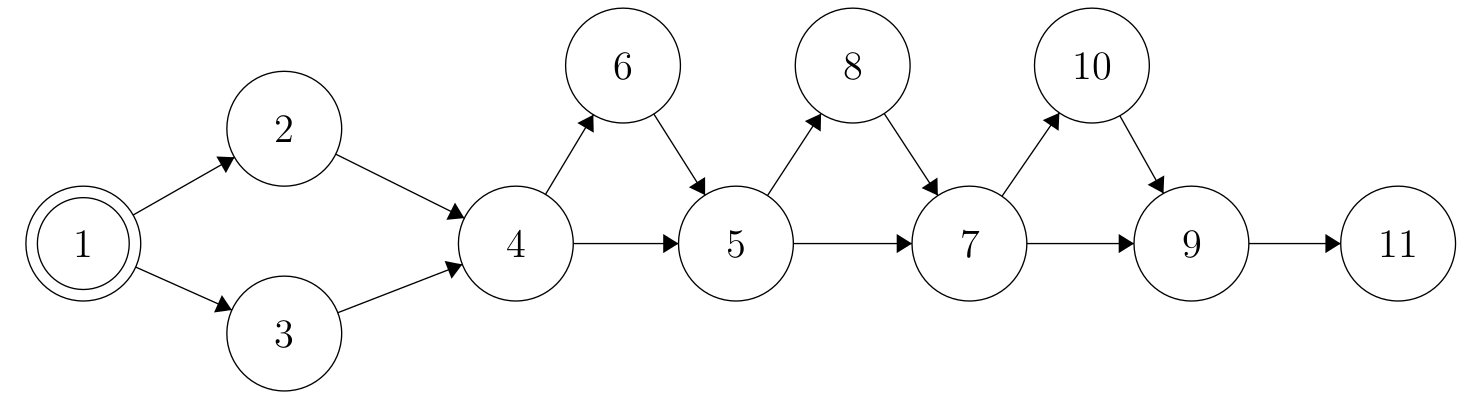
\includegraphics[width=\figwidth\columnwidth]{images/fabrikant/graph.jpg}
	\caption{Fabrikant graph representation}
	\label{fig:fabr_graph}
	\vspace{\figvspace}
\end{figure}

Node 1 represent the only source of traffic, node 4 will prefer to reach the 
destination through node 2, but the link is slower, triggering changes in the
network as required by \cite{fabrikant}.

Taking this base frabrikant graph other 4 graphs has been deveolped, one for each
\ac{MRAI} strategy applyed.

\subsection{Clique Graph}
\label{subsec:clique_graph}

The clique graph used for the clique experiemnts is composed of \num{15} nodes
plus one external node that is the source of a destination.
Each node is connected to every other node in a mesh network. The only node that
does not respect this rule is the destination source. it has only one link 
that is connected to the node of the mesh network number \num{0}.

Relationships between nodes are of the servicer type, so each node has \num{14}
clients to updated when it receives an update.
This ensures that the information is shared in the entire network.

For this network has been generated one graph for each fixed \ac{MRAI} used, so
that at the end we had \num{60} different clique graphs with the correct timer value
equal on each link.

\subsection{Internet Like Graph}
\label{subsec:internet_graph}

This network is composed of \num{100} nodes, it is not enough to emulate the Internet
but, with enough computation time, the results should be comparable with bigger graphs.
The graph has been produced following \cite{elmokashfi}.

In the graph has been chosen only one node that shares a destination.
The node has been chosen randomly in the set of clients nodes.

For each experiment, depending on the type of \ac{MRAI}, a new graph file has
been generated with different \ac{MRAI}s values on the edges.

In total has been generated \num{10000} internet like graphs.

The base graph is represented in \Cref{fig:internet_like_graph}. The figure
include two different layout of the graph, to show the hierarchical structure.
Central nodes (red nodes) represent the tier one nodes, and them compose a little
mesh network at the highest level of the network.
Other types of nodes could be M, CP or C, the las category is the one representing
the clients that can't do peering with other nodes and them are the magiority
of the nodes.
The random node that share a destination is chosen in the C set.

\begin{figure}[tb]
	\centering
	\begin{subfigure}{\columnwidth}
		\centering
		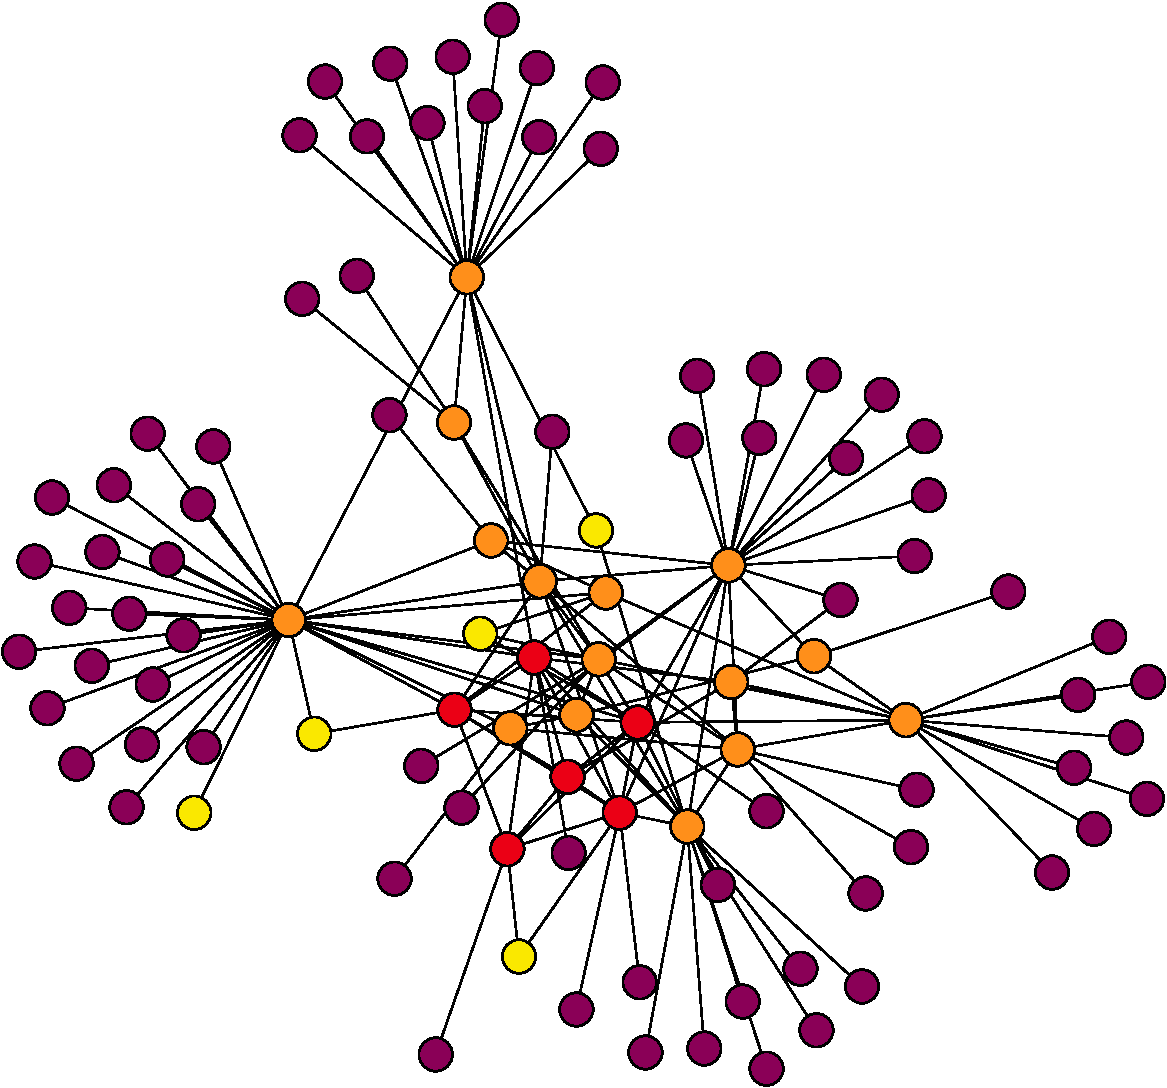
\includegraphics[width=\figwidth\columnwidth]{images/internet_like/graph-100-colored}
		\caption{Internet like graph with an "explosive" layout}
		\label{fig:internet_like_graph_explosive}
		\qquad
	\end{subfigure}

	\begin{subfigure}{\columnwidth}
		\centering
		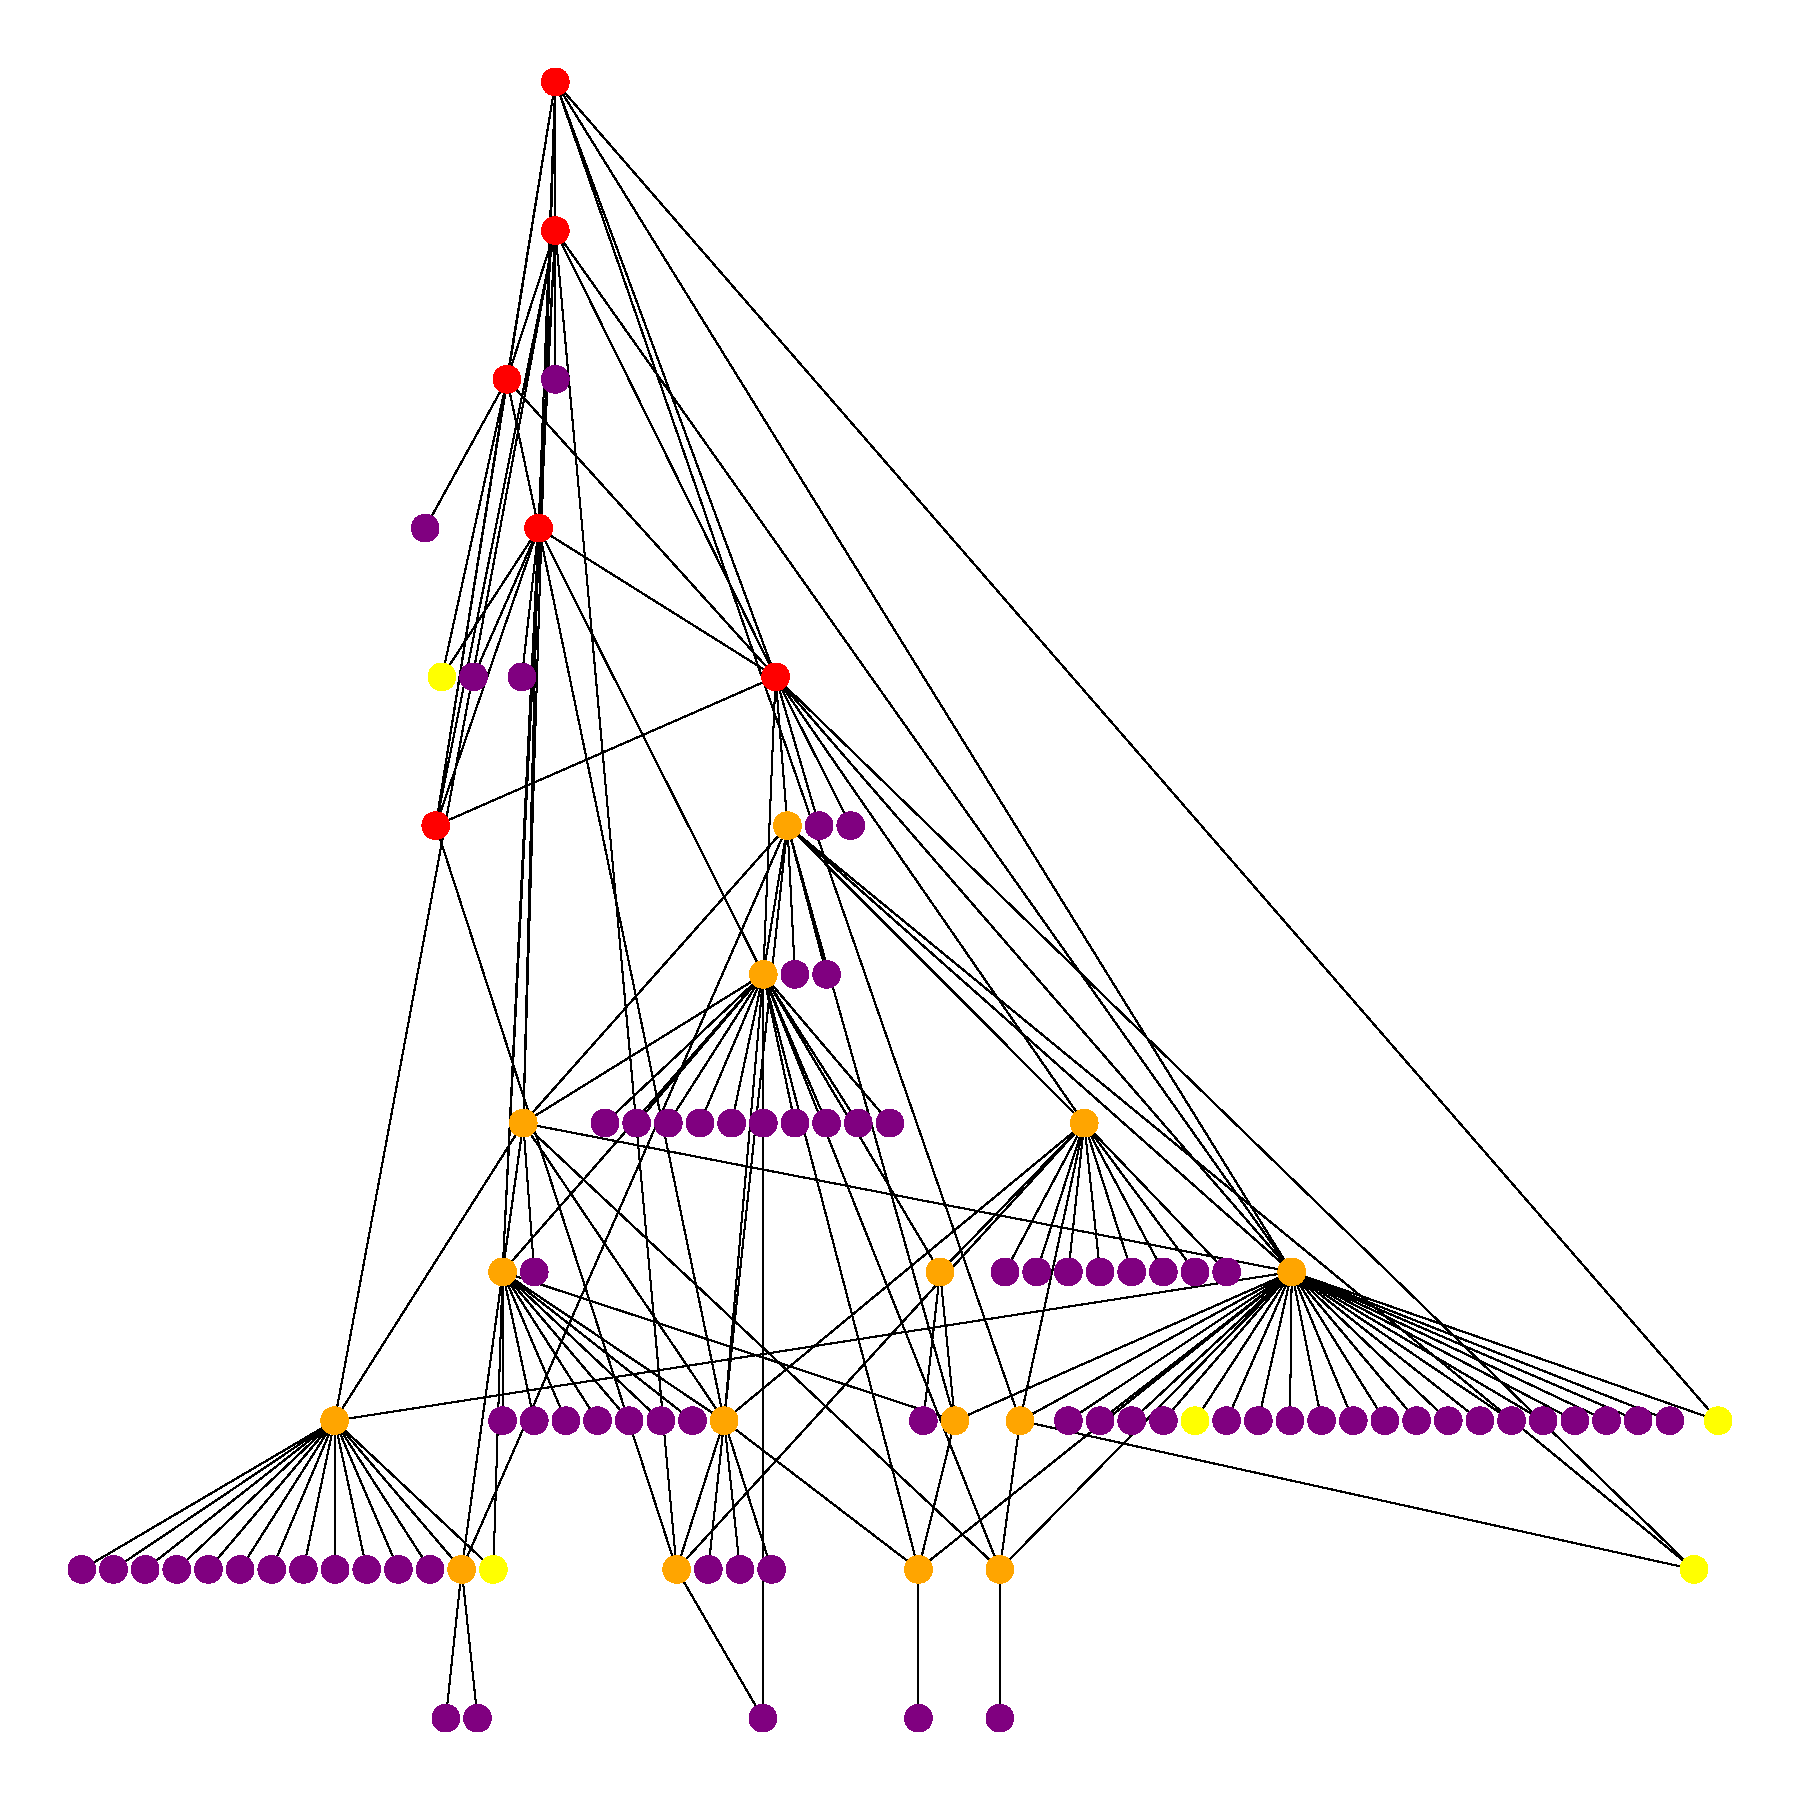
\includegraphics[width=\figwidth\columnwidth]{images/internet_like/graph_dot}
		\caption{Internet like graph with a "hierarchical" layout}
		\label{fig:internet_like_graph_hierarchical}
		\qquad
	\end{subfigure}

	\caption{Internet like graph colored to show the hierarchicaly structure, 4 tipes
			 of nodes, T (tier 1 mesh), M, CP, C (Customers, purple one)}
	\label{fig:internet_like_graph}
	\vspace{\figvspace}
\end{figure}

\section{Input arguments}
\label{sec:envDesc}

In this section are described the inputs arguments used for the different environments.

\subsection{Fabrikant arguments}
\label{sec:fabrikant_arguments}

\begin{itemize}
	\item seeds: \num{20} different seeds;
	\item Signaling: "AWA", The input signal determines the messages that 
		the source should send
	\item Implicit withdraw: active
	\item Withdraw distributions: \num{3} different withdraw uniform distributions
		$[5, 10]$, $[10, 15]$ and $[30, 45]$
	\item Reannouncement distributions: \num{3} different announcement uniform distributions
		$[5, 10]$, $[10, 15]$ and $[30, 45]$
	\item Processing time: constant with value \num{0.00001}
	\item Network delay: \num{3} uniform distributions in $[0.001, 1]$, $[0.5, 3]$ and $[2, 6]$
\end{itemize} 

The number of possible different combinations of these values is \num{540}, so 
for each different \ac{MRAI} type has been done \num{540} experiments and
in total \num{2160} expieriments in the fabrikant environment.

\subsection{Clique arguments}
\label{subsec:clique_arguments}

\begin{itemize}
	\item seeds: \num{10} different seeds;
	\item Signaling: "AW" 
	\item Implicit withdraw: active
	\item Withdraw distributions: uniform distribution $[5, 10]$
	\item Reannouncement distributions: Ininfluent 
	\item Processing time:i uniform distribution $[0.01, 1]$ 
	\item Network delay: uniform distribution in $[0.012, 0.1]$
\end{itemize} 

This environment attempt to replicate what has been presented in \cite{griffin2001experimental}

In total this environment would run 10 different permutations because the only
element that can differ is the input seed.
But has been done in a total of \num{61} experiments changing the \ac{MRAI} value between
$0$ and $60$, so in total, we had \num{610} runs, \num{10} for each \ac{MRAI} value.
It wouldn't have much sense, in my opinion, to run more than one simulation batch per
\ac{MRAI} value, because the repetition of the seed with no difference in any
other parameter would have produced the same result.
For comparison purposes the same environemnt has been run even with the 
implicit withdraw option deactivated.

\subsection{Internet like arguments}
\label{subsec:internet_like_arguments}

\begin{itemize}
	\item seeds: \num{10} different seeds;
	\item Signaling: "A" 
	\item Implicit withdraw: active
	\item Withdraw distributions: Ininfluent
	\item Reannouncement distributions: Ininfluent 
	\item Processing time: constant with value \num{0.00001}
	\item Network delay: uniform distribution in $[0.012, 3]$
\end{itemize} 

The environment has been used for random experiments and fixed mrai experiments.

Like in the clique experiments, in the case of the fixed \ac{MRAI}, every link
had the same timer value.
But this time has been used also fractions of seconds to highlight the trend.
There have been \num{121} experiments with \ac{MRAI} in the ensemble $[0.0, 60]$.
In the first fraction $[0.0, 5.0]$ has been used a step of \num{0.1} doing \num{51}
experiments.
The second fraction was $[5.5, 20]$ with a step of \num{0.5}, doing in total \num{30}
experiemnts.
The last subset was $[21, 60]$ with a step of \num{1}, doing in total \num{40}
experiments.
The final total is \num{121} experiments and for each of them has been done
\num{10} runs, one for each possible seed of the environment.

For comparison purposes the same environemnt has been run even with the 
implicit withdraw option deactivated.

The second type of experiments with the internet like environemnt were run
with the \ac{DPC} \ac{MRAI} strategy.
This centrality metric si explained in \Cref{sec:dpc}, it's applyed on every
edge of the network considering three phases in the graph.
Then I applyed the same $MRAI_{mean}$ sequence that was described for the
constant \ac{MRAI} experiments, so in total we have \num{121} experiments.

For comparison purposes the same environemnt has been run even with the 
implicit withdraw option deactivated.

The last type of experiments with the internet like environment were run 
with random graphs.
Before running a random experiment the $MRAI_{mean}$ were chosen randomly before
the generation of the random graph.
In total has been chosen \num{100} random $MRAI_{mean}$ uniformly distributed
in the set $[0, 60]$ the limit \num{60} has been chosen arbitrarily being the
double of the actual standard.
\num{100} random graphs were generated for each $MRAI_{mean}$.
Each link would obtain a random value in the set $[0, 240]$ and then all the
values would be re-proportioned to respect the $MRAI_{mean}$
At the end for each random graph would be done \num{10} runs thanks to the 10 
different seeds.
The total number of this particular configuration is $100*100*10$ equal to 
\num{100000} single runs.

\section{Destination Partial Centrality}
\label{sec:dpc}

In this section I will define and explain how was applyed the \ac{DPC} in the
experiments.
What follow has been taken from \cite{milani2020improving}.

The intuition at the base of centrality-based \ac{MRAI} tuning is that we would 
like \ac{MRAI} to increase in the initial phase, close to Tier one nodes set (from now on \tr set),
and then, when the core of routers around \tr stabilized, it should start decreasing in 
order to quickly propagate the new stable situation to the rest of the Internet. 
To verify the validity of this intuition we set-up a strategy that exploits  
the previous knowledge of the network graph together with the concept of \acf{DPC}.

\ac{DPC} is a variant of so-called load centrality which is defined in its general 
form as follows \cite{Brandes2008Variants}: Consider a graph \graph and an 
algorithm to identify the (potentially multiple) minimum weight path(s) between 
any pair of vertices $s,d$.
Let $\theta_{s,d}$ be a quantity of a generic commodity that is sent from vertex
$s$ to vertex $d$.
We assume the commodity is always passed to the next hop following the minimum weight paths.
In case of multiple next hops, the commodity is divided equally among them.
We call $\theta_{s,d}(v)$ the amount of  commodity forwarded by vertex $v$.
The \emph{load centrality} of $v$ is then given by:
\begin{equation}
LC(v) = \sum_{s,d \in \nodeset}\theta_{s,d}(v)
\label{eq:lc}
\end{equation}

\ac{DPC} adapts load centrality to represent the propagation of routes in an IP network. 
In \ac{DPC} \textit{load} represents the amount of networks that a BGP node exports. 
Not all nodes that run BGP generate \textit{load}, but all nodes that forward traffic 
have a non-zero DPC centrality. We call $\destinationset \subseteq \nodeset$ the 
set of nodes that can be source and/or destination of traffic (they export at least one network) 
and $N_s, N_d$ the number of networks that are exported by node $s$ and $d$, 
respectively, then $\theta_{s,d} = \frac{N_s + N_d}{2}$. \ac{DPC} $\Delta(v)$ of 
any vertex $v\in \nodeset$ is defined as
\begin{equation}
\dpc(v) = \sum_{s,d\in \pathset} \theta_{s,d} (v)
\label{eq:dpcv}
\end{equation}

With DPC we model the fact that some Internet routers export network addresses, 
and for this reason they generate changes in the network state, while other routers 
only forward traffic, but still their centrality can be larger than zero.

In a previous work we have shown that load centrality can be computed in a distributed 
way with minimal modifications to a Distance-Vector routing protocol. We also experimentally 
verified that computing \ac{DPC} is possible with a custom BGP extension, and thus, 
it can be incrementally deployed on the Internet without requiring any global 
coordination 
\footnote{A brief explanation on how to calculate in a distributed way the centrality 
can be found at: \url{https://iof.disi.unitn.it/docs/DPConTopOfBGP.pdf}}.
Further theoretical details are outside the scope of this paper, but principles 
of centrality-based routing can be found in\,\cite{MaLo18_ToN,GhiMa18_infocom}.

Our proposal configures \ac{MRAI} as a function of \ac{DPC} with the following 
model: We assume the information contained in the \update message propagates in 
the network in three phases, which identify three propagation graphs:
\begin{itemize}
    \item \textit{\textbf{Ascending phase graph \ascentgraph}:} made by the 
		nodes updated without reaching tier one nodes;
    \item \textit{\textbf{Tier one graph \tiergraph}:} made by tier-1 nodes;
    \item \textit{\textbf{Descending graph phase $\descentgraph = \graph - \ascentgraph - \tiergraph$}:} 
		the rest of the graph.
\end{itemize}

Considering a graph-wide maximum timer $T=\SI{30}{\second}$ and \ac{DPC} 
$c_i\in [0,1]$ for node $i$, DPC-based \ac{MRAI} $T_{ij}$ used by node $i$ 
with neighbor $j$ is set as follows:
\begin{equation}
    T_{ij}=
    \begin{cases}
    \frac{T}{2}c_i & \forall i\in \ascentnodeset  \\
    \frac{T}{2} & \forall i\in \tiernodeset \\
    \frac{T(1-c_i)}{2}+\frac{T}{2} & \forall i\in \descentnodeset\\
    \end{cases}
\end{equation} 

\section{Experiments Results}
\label{sec:results}

The first results that I would like to examine is the single node
results from the fabrikant experiment.
In \Cref{fig:fabr_30sec_9_signaling,fig:fabr_descendent_9_signaling} are represented
two signalling outputs of the node number \num{9}.

The $x$ axis represents the number of messages in the output signal.
The first $y$ axis, the one on the left, represents the probability to have a certain
number of messages in the output sequence and should be used with "withdraw
messages", "Advertisement messages" and "Total messages" lines.
For example in \Cref{fig:fabr_30sec_9_signaling} we can see that there is a really
high probability to have \num{0} withdraws in the output sequence, and we would never
see more than 1 withdraw by the fact that the "withdraw line" doesn't go over that
value of the $x$ axis.
In the same way, we can read the other lines, for example in the same figure is
possible to see that the more probable output signal is composed by \num{3} messages,
because is the highest point of the blue line.
The second $y$ axis, the one on the right, represents the number of \textbf{unique}
states.
This axis should be used with the line that represents the "possible outputs".
Looking the \Cref{fig:fabr_30sec_9_signaling} is possible to see that for
output signals with \num{6} messages we have more than \num{40} uniques output
states.

Knowing that the output signalling is strictly dependent by the input that a 
node receives and the evaluation time of those messages we can already see the
effects of an inconvenient \ac{MRAI} setting.
In \Cref{fig:fabr_descendent_9_signaling} there are a lot more output states.
In those experiments we reach event output states of length \num{16} and the 
probability to have at least one withdraw is higher to the probability to 
don't have one.
Knowing that the implicit withdraw system is active having one withdraw means
that the node has no other possibilities to withdraw the network not knowing any
other path.

\begin{figure}[tb]
	\centering
	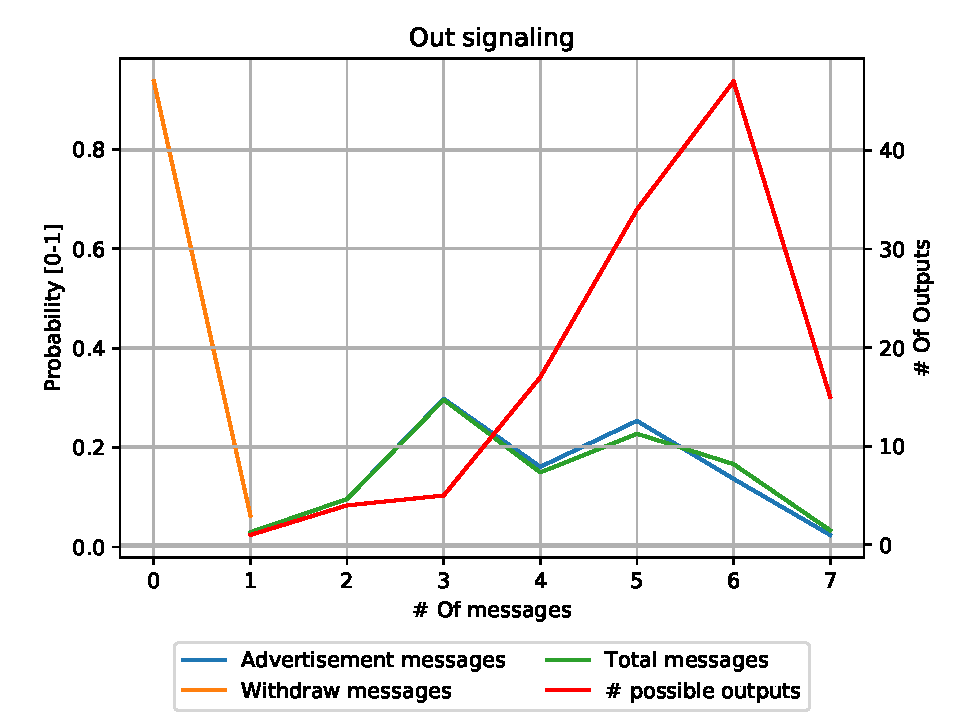
\includegraphics[width=\figwidth\columnwidth]{images/fabrikant/fabrikant-30fixed/results_9_signaling_nmessage_prob}
	\caption{Fabrikant MRAI fixed 30 seconds, node 9 signalling output}
	\label{fig:fabr_30sec_9_signaling}
	\vspace{\figvspace}
\end{figure}

\begin{figure}[tb]
	\centering
	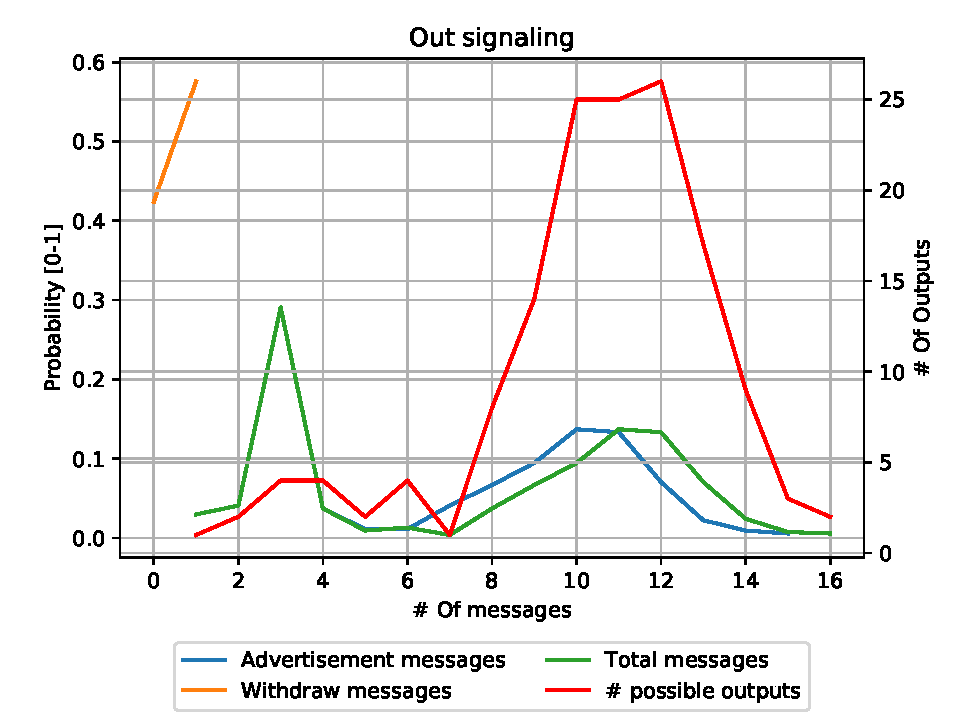
\includegraphics[width=\figwidth\columnwidth]{images/fabrikant/fabrikant-descendent/results_9_signaling_nmessage_prob}
	\caption{Fabrikant MRAI descendent, node 9 signalling output}
	\label{fig:fabr_descendent_9_signaling}
	\vspace{\figvspace}
\end{figure}

Like we said before we used 4 different \ac{MRAI}s strategies in the fabrikant
environment, and them are compared in the \Cref{fig:fabr_conv_time_comp,fig:fabr_msg_comp}.
The no mrai method is strictly dependent on delays and other events of the network
and is possible to see that it has the smallest convergence time but with the higher
number of messages necessary to reach the convergence.
The \num{30} seconds strategy could be the slowest one because if something goes
wrong is necessary to wait a long time to repair the damage, but it wouldn't
require too many messages on the other side.
The descendant method seems a good solution on the convergence time side, but
on the other side, like is described in \cite{fabrikant} it could easily lead
to a lot of messages.

\begin{figure}[tb]
	\centering
	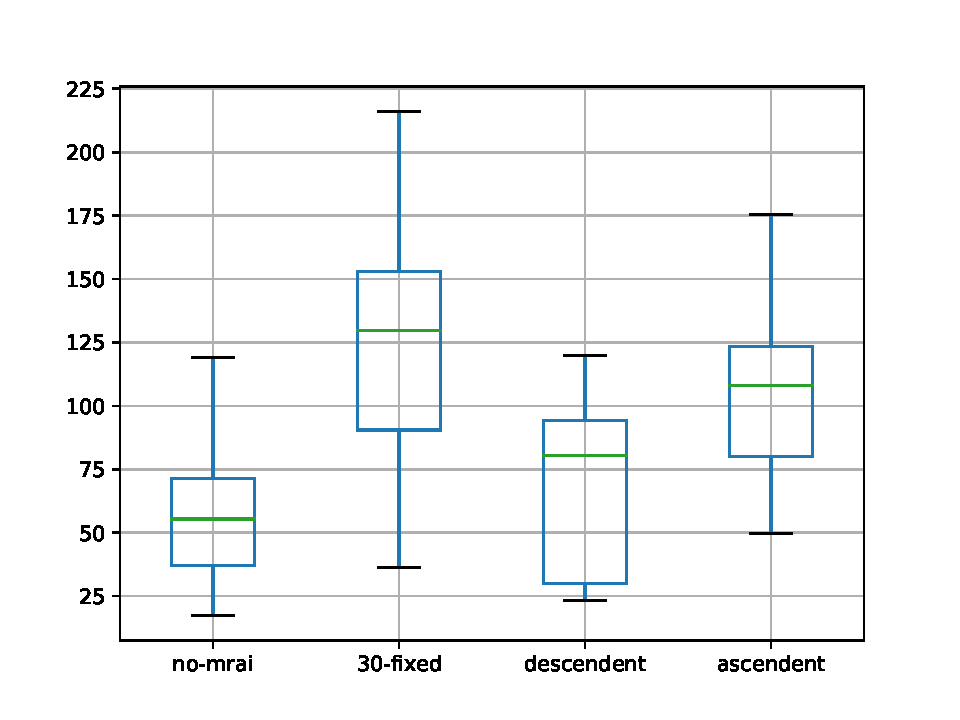
\includegraphics[width=\figwidth\columnwidth]{images/fabrikant/convergence_time}
	\caption{Fabrikant experiments convergence time comparison}
	\label{fig:fabr_conv_time_comp}
	\vspace{\figvspace}
\end{figure}

\begin{figure}[tb]
	\centering
	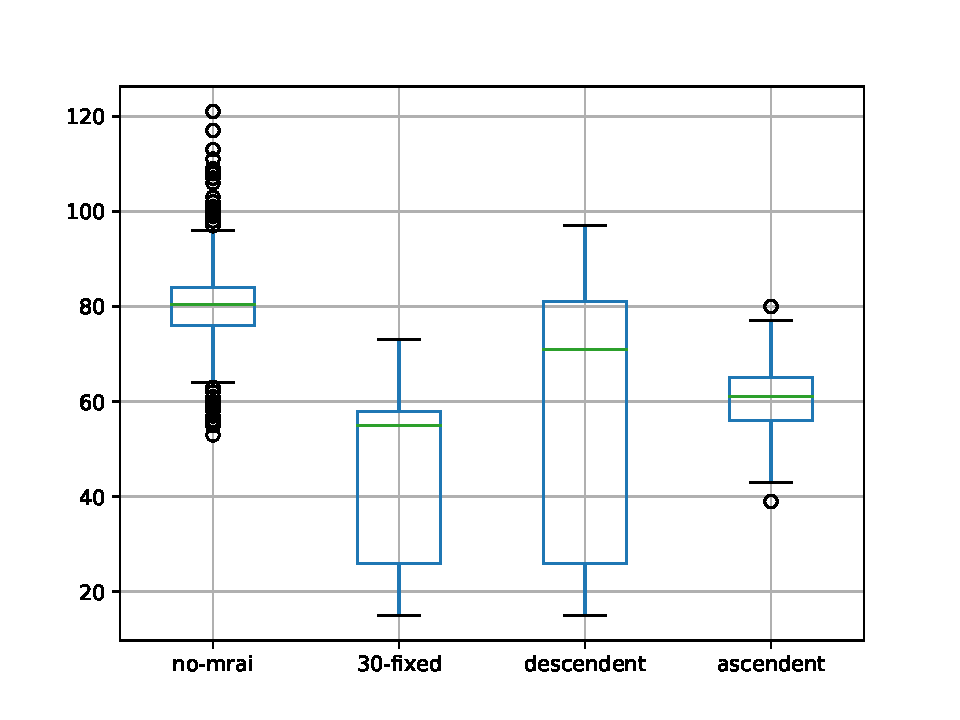
\includegraphics[width=\figwidth\columnwidth]{images/fabrikant/messages_comparison}
	\caption{Fabrikant experiments number of messages comparison}
	\label{fig:fabr_msg_comp}
	\vspace{\figvspace}
\end{figure}

In \Cref{fig:clique_pareto_freq,fig:clique_mrai_evolution} are reported the general
network results obtained in the clique environment.
The goal of this study is to see in a general way how \ac{MRAI} could influence
even a small network as this clique of \num{15} nodes.

In \Cref{fig:clique_pareto_freq} every point of the plot is the mean of the \num{10}
runs executed with a fixed \ac{MRAI}.
On the $x$ axis is represented the number of messages correlated with the convergence
time on the $y$ axis.
The red points are the Pareto front of the set of all points.
We can see from the plot that a lot of experiments has a mean of messages sent 
around \num{2000} independently from the \ac{MRAI} so we can guess that after
a threshold of \ac{MRAI} the number of messages stabilizes around that value.
On the other side, before this threshold we can guess there is a lot of variance
in the number of messages but the mean convergence time is similar.
These guesses are confirmed by the \Cref{fig:clique_IW_mrai_evolution} where we can clearly
see those trends.
The two $y$ axis are used to represent the trend of the convergence time and
the number of messages transmitted in relation of the \ac{MRAI} value.
The two \Cref{fig:clique_IW_mrai_evolution,fig:clique_noIW_mrai_evolution} refers
to two different situations in the same clique graph.
In the first figure the implicit withdraw is active, in the second has been
deactivated, the difference is evident, the number of messages and the convergence
time are higher without the implicit withdraw active, and also take a longer time
to reach a stable point in \Cref{fig:clique_noIW_mrai_evolution}. 
This confirm what has been presented in \cite{labovitz2000delayed}.

\begin{figure}[tb]
	\centering
	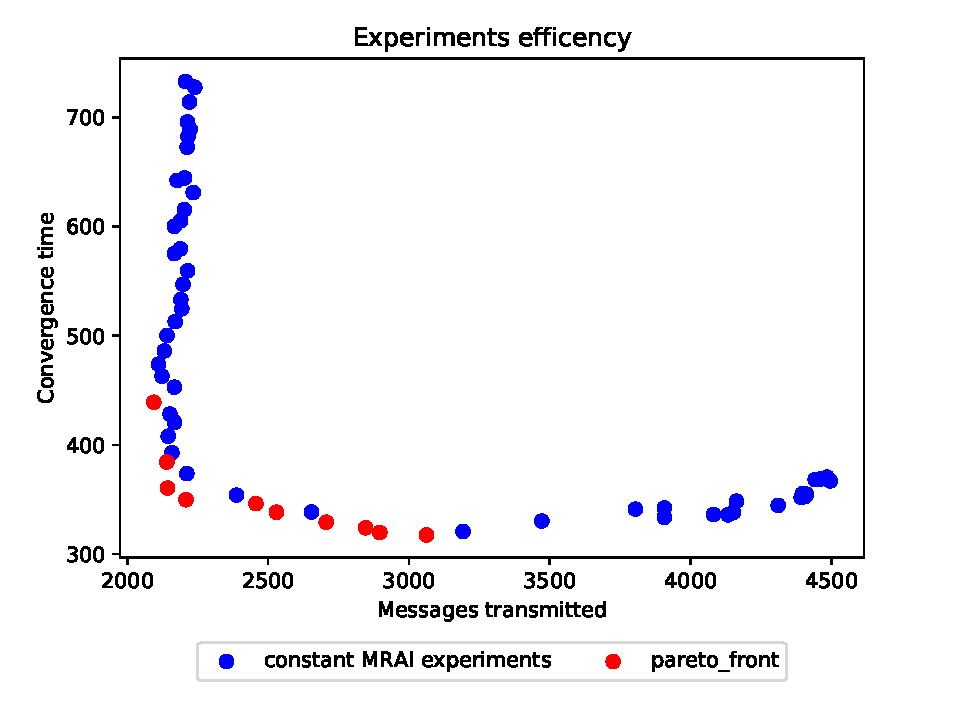
\includegraphics[width=\figwidth\columnwidth]{images/clique/pareto-clique-constant}
	\caption{Pareto front in the clique environments}
	\label{fig:clique_pareto_freq}
	\vspace{\figvspace}
\end{figure}

\begin{figure}[tb]
	\centering

	\begin{subfigure}{\columnwidth}
		\centering
		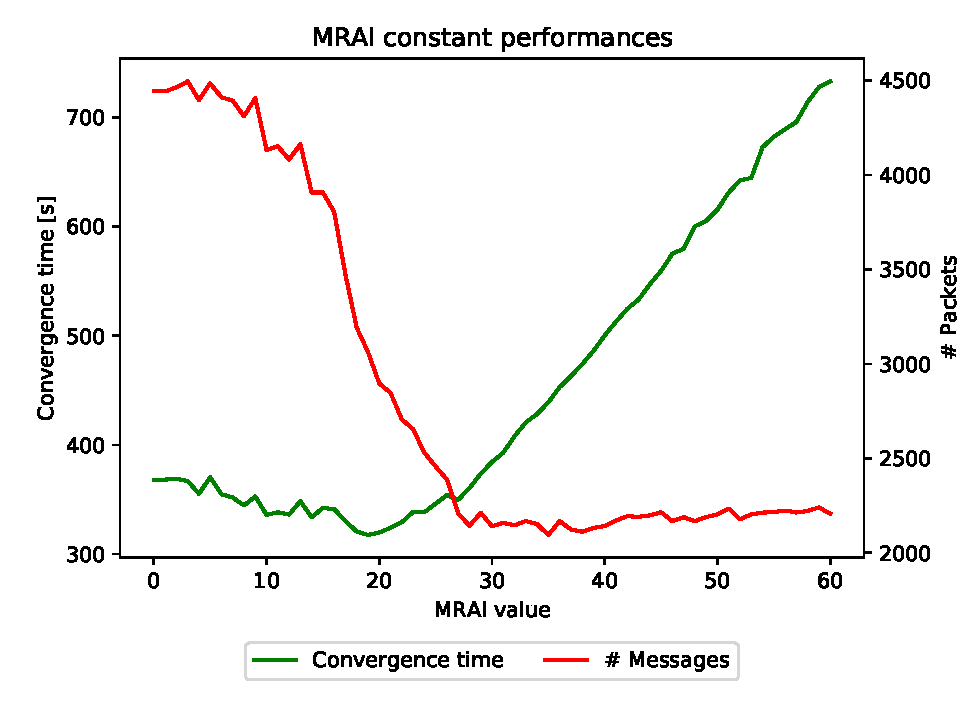
\includegraphics[width=\figwidth\columnwidth]{images/clique/mrai_evolution}
		\caption{Clique environment with Implicit Withdraw active}
		\label{fig:clique_IW_mrai_evolution}
		\qquad
	\end{subfigure}

	\begin{subfigure}{\columnwidth}
		\centering
		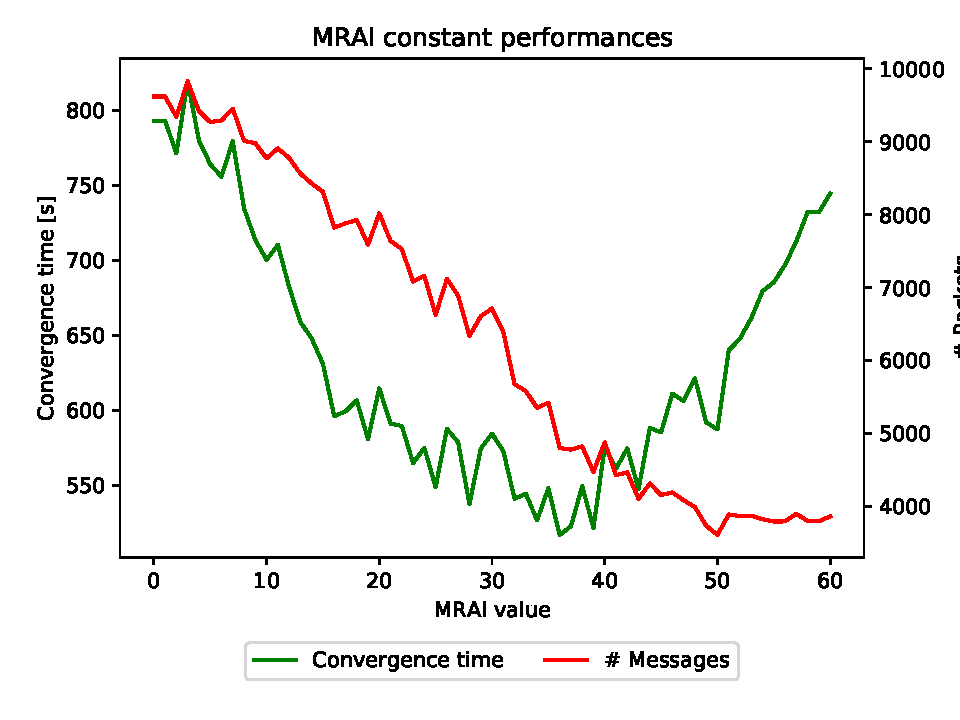
\includegraphics[width=\figwidth\columnwidth]{images/clique-noImplicitWithdraw/mrai_evolution}
		\caption{Clique environment \textbf{without} Implicit Withdraw active}
		\label{fig:clique_noIW_mrai_evolution}
		\qquad
	\end{subfigure}

	\caption{Evolution of the number of messages sent and the convergence time as \ac{MRAI} grows
		in the clique environment}
	\label{fig:clique_mrai_evolution}
	\vspace{\figvspace}
\end{figure}

On the same environemnt I have produced also two more plots that are presented
in \Cref{fig:clique_mrai_evolution_std}, the plots represent the same trend of
\cref{fig:clique_mrai_evolution} but this time there is a range around 
the lines that represent the standard deviation of every experiment (each experiment
point is the mean of 10 runs).
In \Cref{fig:clique_IW_mrai_evolution_std} is possible to see that with a small
\ac{MRAI} the standard deviation is higher respect to the standard deviation
after a certain threshold of \ac{MRAI}.
The standard deviation of both messages and convergence time seems to be constant
after a certain threshold.
In \Cref{fig:clique_noIW_mrai_evolution_std} is not possible to see clearly the
same trend in the standard deviation, but with an \ac{MRAI} higher than \num{50}
is possible to guess that the standard deviation is starting to be more constant.
\Cref{fig:clique_noIW_mrai_evolution_std} confirms another time that 
without the implicit withdraw the number of messages and the convergence time
would be a lot more suceptible and unpredictable.

\begin{figure}[tb]
	\centering

	\begin{subfigure}{\columnwidth}
		\centering
		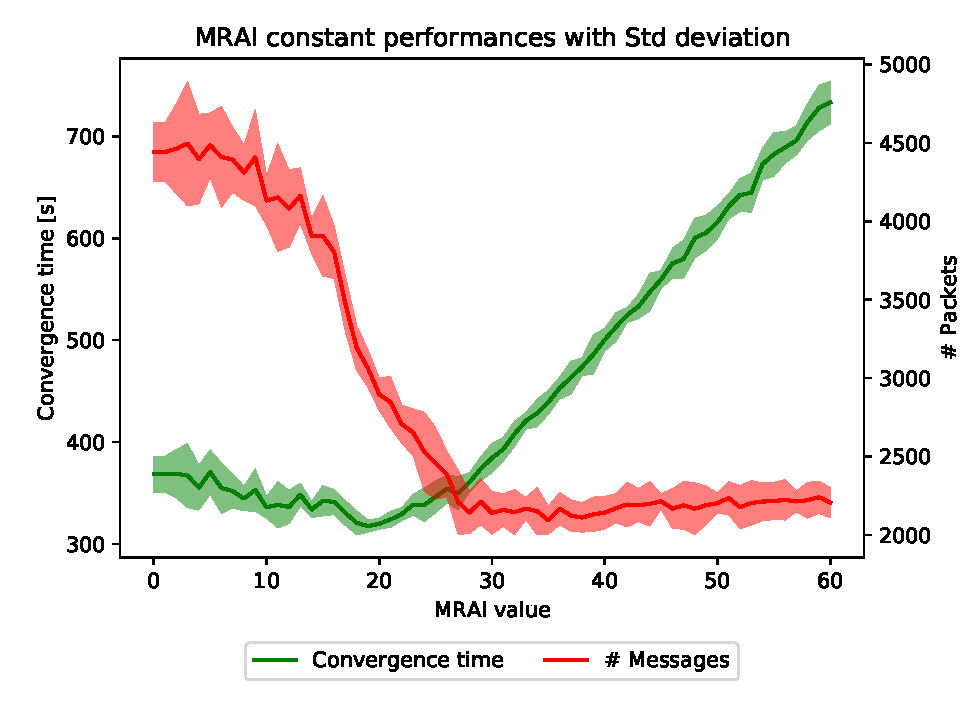
\includegraphics[width=\figwidth\columnwidth]{images/clique/mrai_evolution_std_alpha}
		\caption{Clique environment with Implicit Withdraw active}
		\label{fig:clique_IW_mrai_evolution_std}
		\qquad
	\end{subfigure}

	\begin{subfigure}{\columnwidth}
		\centering
		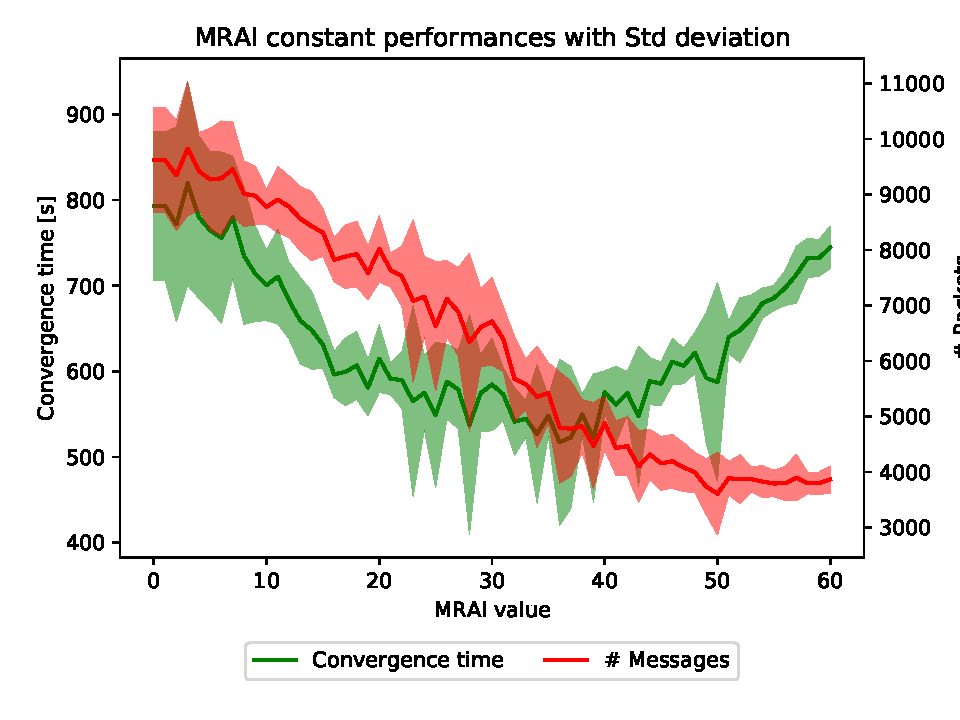
\includegraphics[width=\figwidth\columnwidth]{images/clique-noImplicitWithdraw/mrai_evolution_std_alpha}
		\caption{Clique environment \textbf{without} Implicit Withdraw active}
		\label{fig:clique_noIW_mrai_evolution_std}
		\qquad
	\end{subfigure}

	\caption{Evolution of the number of messages sent and the convergence time as \ac{MRAI} grows
		in the clique environment, the range around the line represent the standard
		deviation of the experiment}
	\label{fig:clique_mrai_evolution_std}
	\vspace{\figvspace}
\end{figure}

The next experiment that I would like to study uses the fixed \ac{MRAI} strategy
on the internet like environment.
The two \Cref{fig:constant_mrai_pareto_freq,fig:constant_mrai_evolution} have the
same structure of the clique results but this time we can see a lot fewer messages
transmitted to reach the convergence.
Also this time we can see in \Cref{fig:constant_mrai_pareto_freq} that a lot of
experiments are concentrated in the range between \num{146} and \num{147} messages
with a high variance on the convergence time.
In fact, we can see from \Cref{fig:constant_mrai_evolution} that the trend is similar
to the one that we saw in the clique graph, but this time the "\# Messages" line
has a steep fall, it reaches the constant state in few seconds (the clique experiment
in \Cref{fig:clique_mrai_evolution} took more than \num{20} seconds).
But we can say the same thing for the convergence time too.
Tose results are similar to the one available in \cite{griffin2001experimental}.
With an \ac{MRAI} lower than \SI{1}{\second} the number of messages could have huge
spikes because the network delay is more influent than the timer.
In fact, after a certain \ac{MRAI} threshold the network delay becomes ininfulent
and the number of messages strictly depend on the order of events that can 
produce constructive messages or disruptive that will be corrected in the next
\ac{MRAI} cicle.
And this is the reason for the constant growing of the convergence time,
it will takes always a higher time to correct incorrect messages.

The trend showed \Cref{fig:constant_IW_mrai_evolution,fig:constant_noIW_mrai_evolution}
is comparable, in \Cref{fig:constant_noIW_mrai_evolution} we can see that
it requires more messages to reach the convergence but not more time.
And the message trend took more time to become stable.

\begin{figure}[tb]
	\centering
	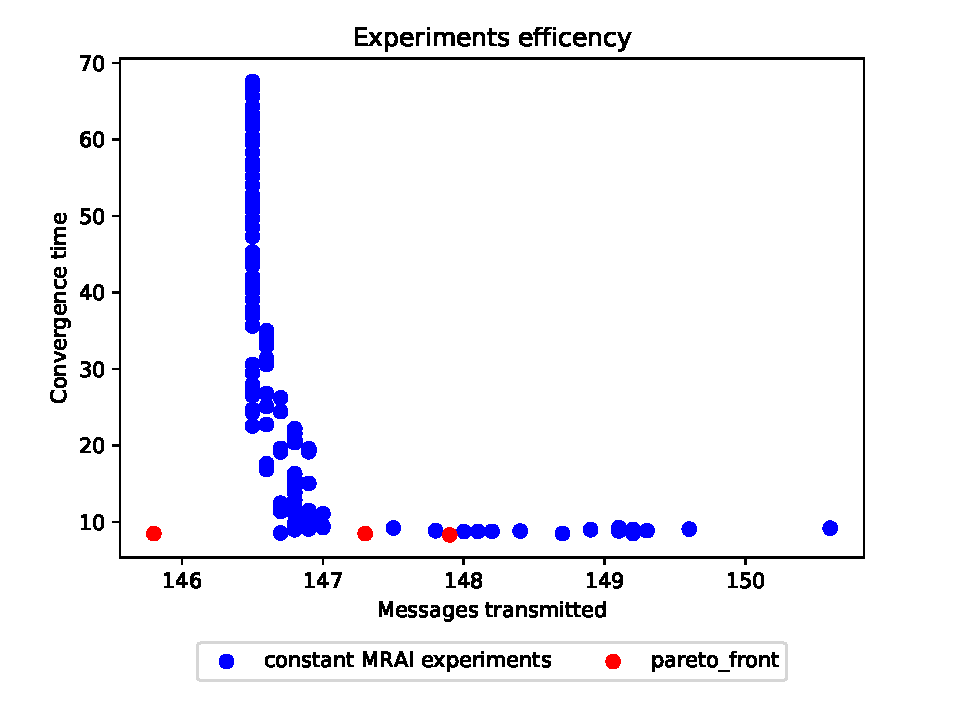
\includegraphics[width=\figwidth\columnwidth]{images/internet_like/graph-100-constant/pareto-constant}
	\caption{Pareto front in the Internet like constant \ac{MRAI} environment}
	\label{fig:constant_mrai_pareto_freq}
	\vspace{\figvspace}
\end{figure}

\begin{figure}[tb]
	\centering

	\begin{subfigure}{\columnwidth}
		\centering
		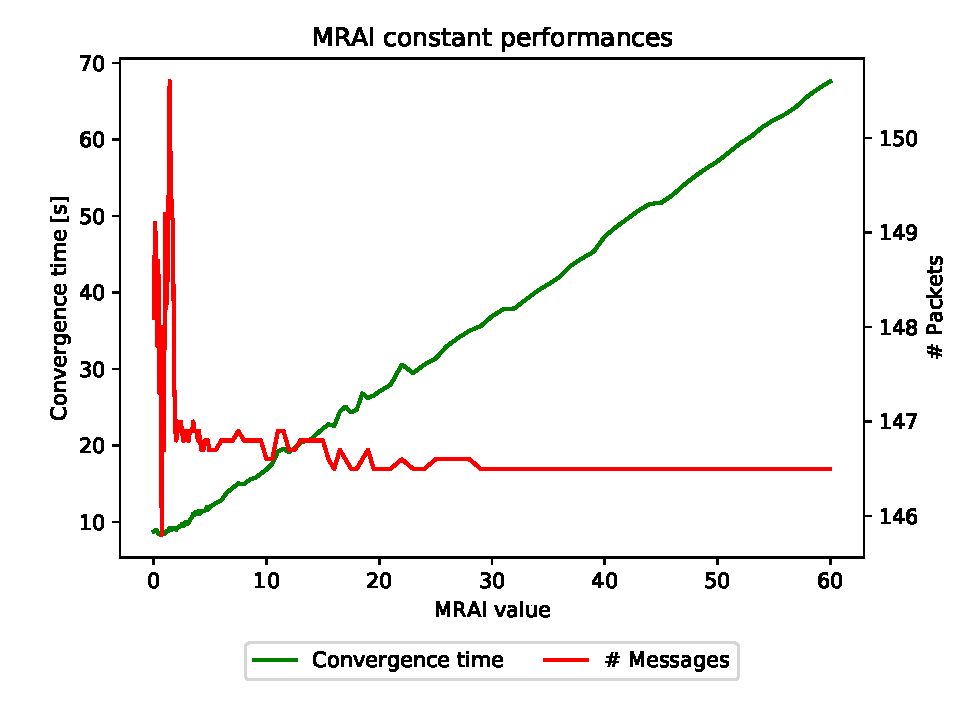
\includegraphics[width=\figwidth\columnwidth]{images/internet_like/graph-100-constant/mrai_evolution}
		\caption{Internet like constant \ac{MRAI} environment with Implicit Withdraw active}
		\label{fig:constant_IW_mrai_evolution}
		\qquad
	\end{subfigure}

	\begin{subfigure}{\columnwidth}
		\centering
		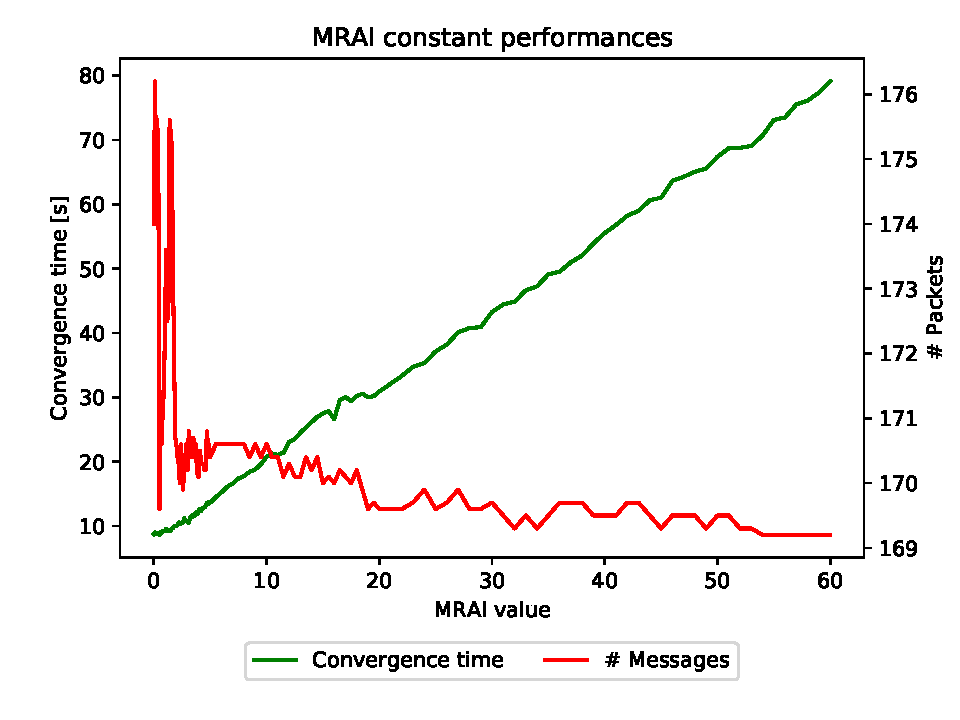
\includegraphics[width=\figwidth\columnwidth]{images/internet_like/graph-100-constant-noIW/mrai_evolution}
		\caption{Internet like constant \ac{MRAI} environment \textbf{without} Implicit Withdraw active}
		\label{fig:constant_noIW_mrai_evolution}
		\qquad
	\end{subfigure}

	\caption{Evolution of the number of messages sent and the convergence time as \ac{MRAI} grows
		in the \textbf{internet like} constant \ac{MRAI} environment}
	\label{fig:constant_mrai_evolution}
	\vspace{\figvspace}
\end{figure}

Like before in \Cref{fig:constant_mrai_evolution_std} is possible to compare the
two techniques (Implicit Withdraw active, vs IW deactivated) with also the 
standard deviation of the experiments.
Each point of the line is the mean of \num{10} runs, the standard deviation
is calculated on those runs, those runs are just a subset of the infinite population
of possible outputs.

The first thing that we can see in both figures is that the standard devition around 
the messages lines is constant for the majority of the time, execpt for a small
\ac{MRAI}s that produces huge spikes of variation.
This effect is caused, like we said before, by the fact that after a certain \ac{MRAI} 
threshold, the order of the events is the only factor that influence the number
of messages. In all this experiments the only thing that changes was the \ac{MRAI}
value, so the order of events is the same (given by the seed of the RNG), and,
given the ininfluence of \ac{MRAI}, produces the same number of output messages
in each run.
It follows that that the standard deviation of each experiment is the same.

We have to remember that with the implicit withdraw feature are produced less
messages by assumption, so we can't compare the number of messages or the standard
variation of those thrends one another.

But, the convergence time is comparable.
We can clearly see that the standard deviation of the time trend in 
\Cref{fig:constant_IW_mrai_evolution_std_a} is lower than the one in 
\Cref{fig:constant_noIW_mrai_evolution_std}.
I guess this difference is caused by the fact that huge storms of withdraws
must be processed and eventually forwarded, causing more computation time
and the forwarding of packets that don't give new knowledge at the neighbors.
Packets that occupy a position in a FIFO link and with a delay.

\begin{figure}[tb]
	\centering

	\begin{subfigure}{\columnwidth}
		\centering
		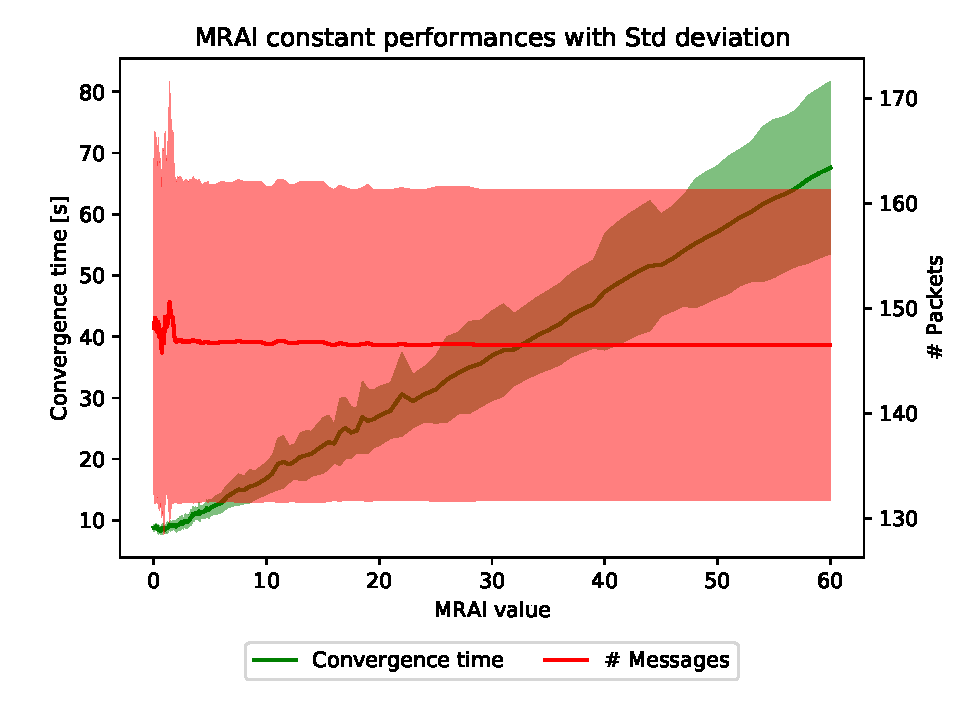
\includegraphics[width=\figwidth\columnwidth]{images/internet_like/graph-100-constant/mrai_evolution_std_alpha}
		\caption{Internet like constant \ac{MRAI} environment with Implicit Withdraw active, standard deviation}
		\label{fig:constant_IW_mrai_evolution_std_a}
		\qquad
	\end{subfigure}

	\begin{subfigure}{\columnwidth}
		\centering
		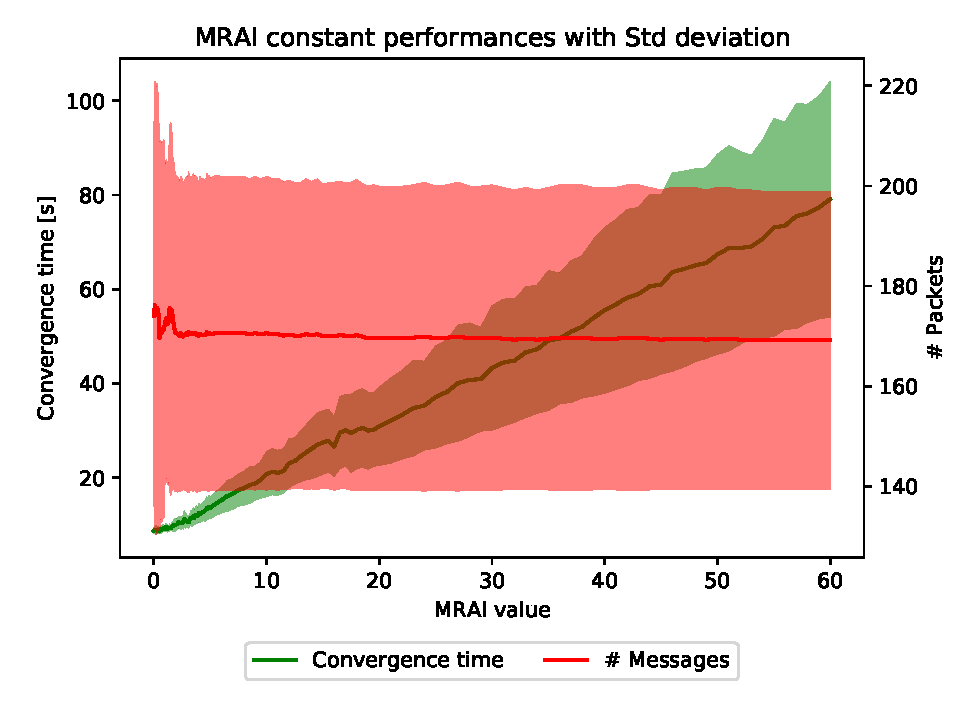
\includegraphics[width=\figwidth\columnwidth]{images/internet_like/graph-100-constant-noIW/mrai_evolution_std_alpha}
		\caption{Internet like constant \ac{MRAI} environment \textbf{without} Implicit Withdraw active, standard deviation}
		\label{fig:constant_noIW_mrai_evolution_std}
		\qquad
	\end{subfigure}

	\caption{Evolution of the number of messages sent and the convergence time as \ac{MRAI} grows
		in the \textbf{internet like} constant \ac{MRAI} environment. The range around the lines
		represent the standard deviation of the experiment}
	\label{fig:constant_mrai_evolution_std}
	\vspace{\figvspace}
\end{figure}

I done the same experiments in the internet like environment with the \ac{DPC}
\ac{MRAI} strategy. The number of experiments and the sequence of $MRAI_{mean}$
tested is the same as the constant \ac{MRAI}.

Is possible to see in \Cref{fig:dpc_mrai_pareto_freq} that the distribution is
similar to the one in \cref{fig:constant_mrai_pareto_freq}, but this
time the spike of vertical values is around the messages value \num{149} with
pratically no variation between one experiment and another.
The horizontal spike this time is on the left of the vertical spike, and this
is important because it represent that is more rare to go over that value of
messages sent.

Like before we can guess that there will be some \ac{MRAI} thresholds for the 
two spikes.

\begin{figure}[tb]
	\centering
	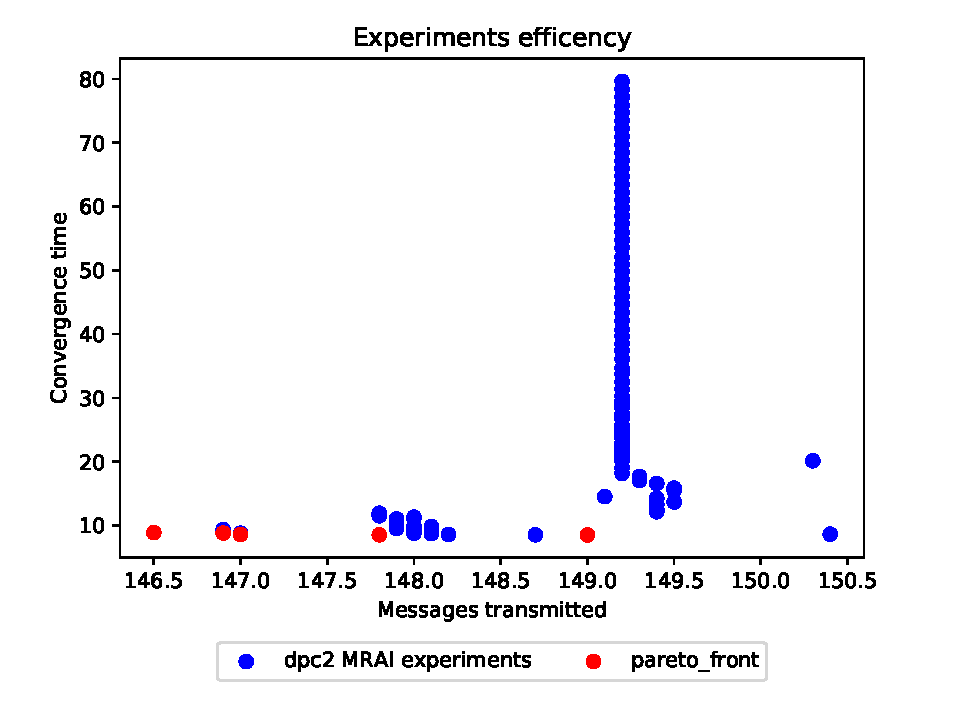
\includegraphics[width=\figwidth\columnwidth]{images/internet_like/graph-100-dpc/pareto-internet_like-dpc}
	\caption{Pareto front in the Internet like \ac{DPC} \ac{MRAI} environment, IW active}
	\label{fig:dpc_mrai_pareto_freq}
	\vspace{\figvspace}
\end{figure}

Once again the guess on the threshold is confirmed by \Cref{fig:dpc_mrai_evolution}
plots where is possible to see that on low \ac{MRAI} values we will have a
huge variation on the number of messages distributed, but once the threshold
is crossed the number of messages will be constant.
And this time if we compare \Cref{fig:dpc_mrai_evolution_IW} with \Cref{fig:constant_IW_mrai_evolution}
we will see that with the \ac{DPC} techinique this threshold is crossed way before.
Is also noticeable that once the threshold is crossed there are no stability issues
on the number of messages.
exept for the \Cref{fig:dpc_mrai_evolution_noIW} plot where we can see some
small variation on the stabilized number of messages.

\begin{figure}[tb]
	\centering

	\begin{subfigure}{\columnwidth}
		\centering
		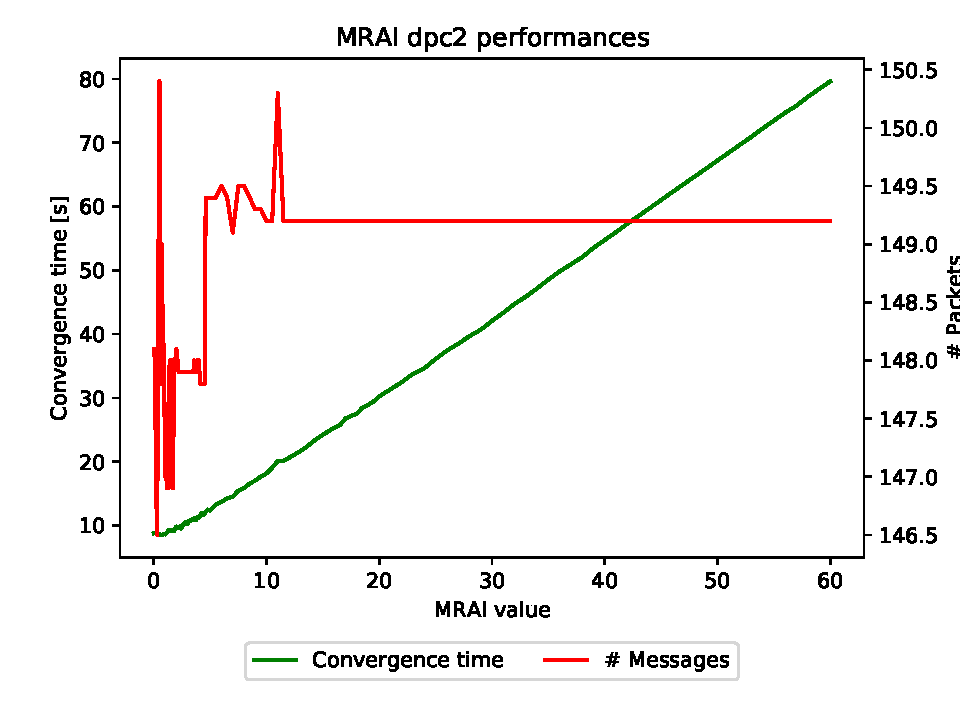
\includegraphics[width=\figwidth\columnwidth]{images/internet_like/graph-100-dpc/mrai_evolution}
		\caption{Internet like \ac{DPC} \ac{MRAI} environment with Implicit Withdraw active}
		\label{fig:dpc_mrai_evolution_IW}
		\qquad
	\end{subfigure}

	\begin{subfigure}{\columnwidth}
		\centering
		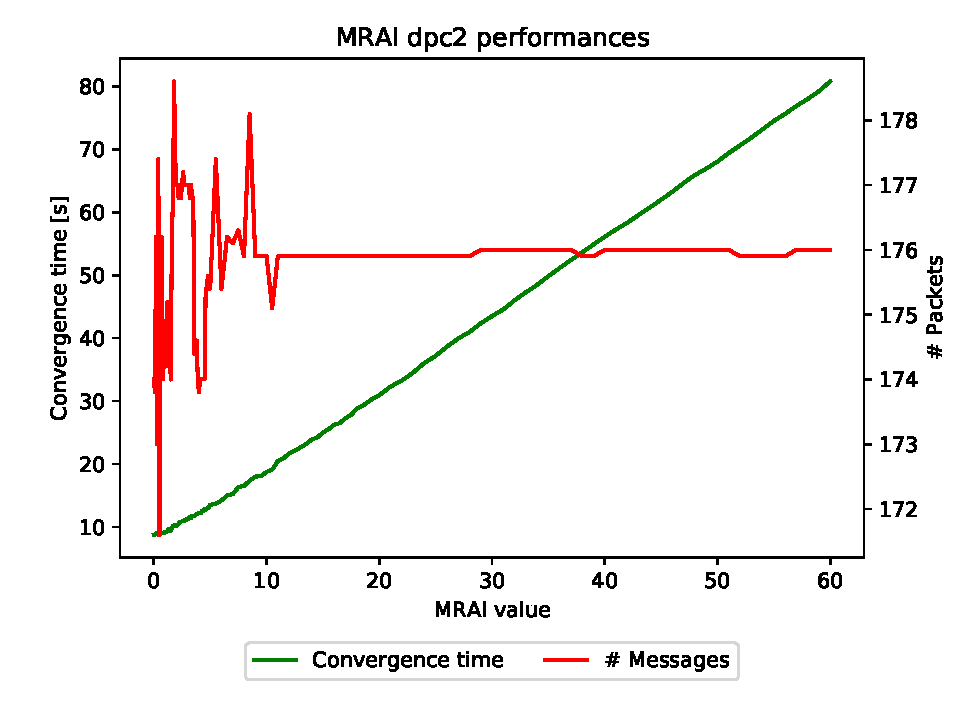
\includegraphics[width=\figwidth\columnwidth]{images/internet_like/graph-100-dpc-noIW/mrai_evolution}
		\caption{Internet like \ac{DPC} \ac{MRAI} environment \textbf{without} Implicit Withdraw active}
		\label{fig:dpc_mrai_evolution_noIW}
		\qquad
	\end{subfigure}

	\caption{Evolution of the number of messages sent and the convergence time as \ac{MRAI} grows
		in the \textbf{internet like} constant \ac{MRAI} environment}
	\label{fig:dpc_mrai_evolution}
	\vspace{\figvspace}
\end{figure}

Like before in \Cref{fig:dpc_mrai_evolution_std} is possible to see the
\ac{DPC} \ac{MRAI} strategy experiments on the internet like evironment with
the standard deviation.

Like before the number of messages has a constant standard deviation after the
threshold thanks to the event sequence.

The two plots respectively in \Cref{fig:dpc_mrai_evolution_IW_std,fig:dpc_mrai_evolution_noIW_std}
are similar one another, execpt for the number of messages transmitted that it's
not comparable.
The big difference that we can see from the constant \ac{MRAI} experiments is that
the standard deviation around the time, in the \ac{DPC} \ac{MRAI} strategy, is 
bigger than the other. An educated guess could be that we can have a lower 
convergence time because \ac{MRAI} is higher only where necessary and correct 
informations would travel faster around the network. On the opposite side 
bad informations could spread too, generating the opposit case with an high
convergence time, caused by the fact that take more time to make every node 
converge.

\begin{figure}[tb]
	\centering

	\begin{subfigure}{\columnwidth}
		\centering
		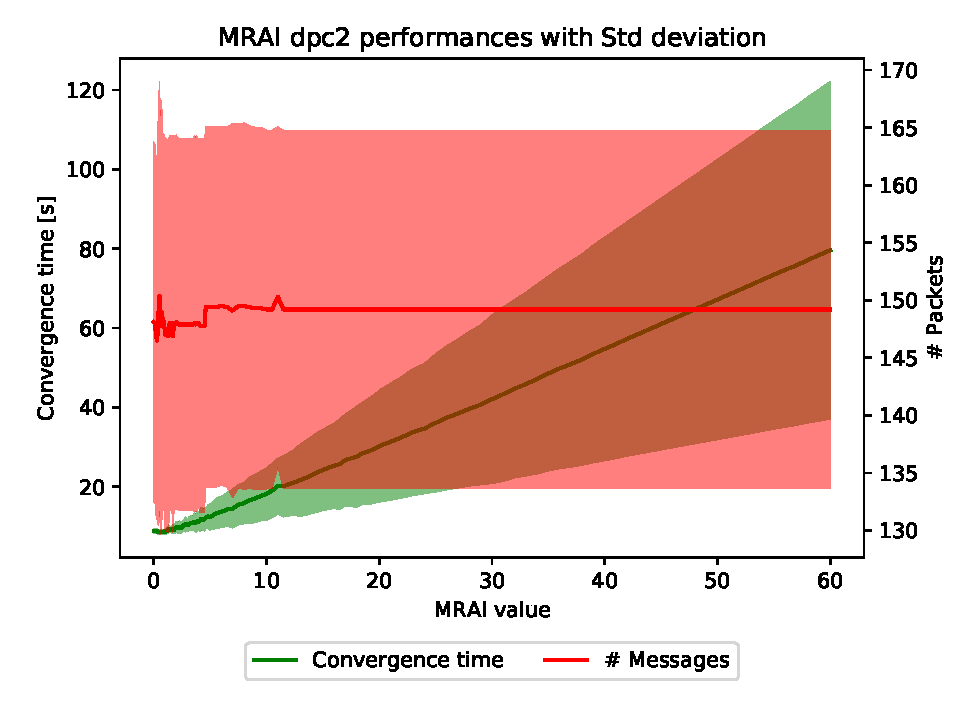
\includegraphics[width=\figwidth\columnwidth]{images/internet_like/graph-100-dpc/mrai_evolution_std_alpha}
		\caption{Internet like \ac{DPC} \ac{MRAI} environment with Implicit Withdraw active, standard deviation}
		\label{fig:dpc_mrai_evolution_IW_std}
		\qquad
	\end{subfigure}

	\begin{subfigure}{\columnwidth}
		\centering
		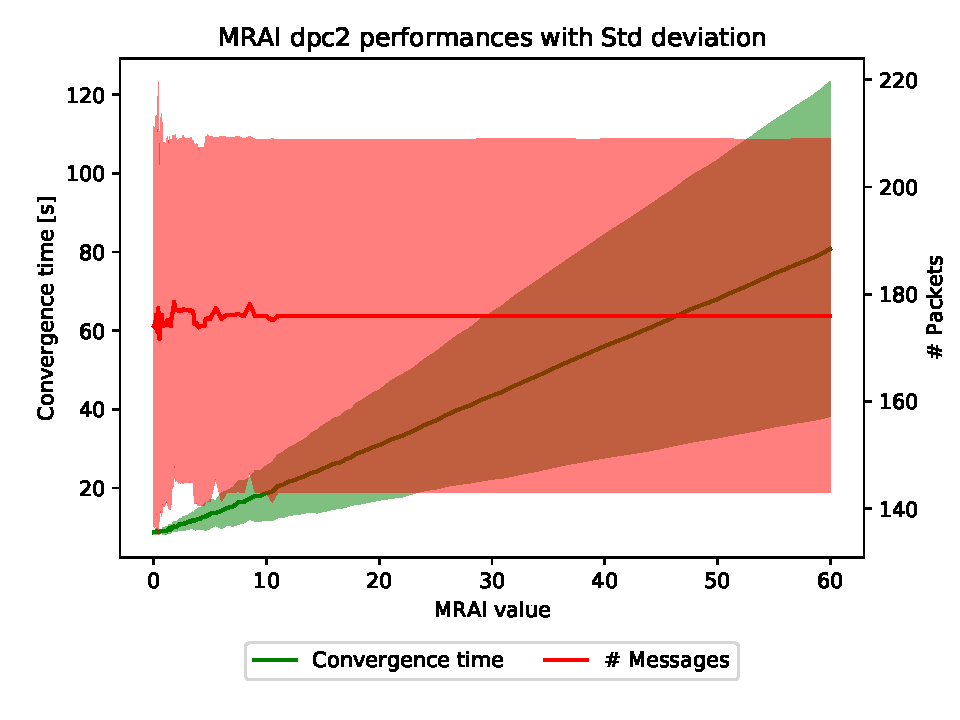
\includegraphics[width=\figwidth\columnwidth]{images/internet_like/graph-100-dpc-noIW/mrai_evolution_std_alpha}
		\caption{Internet like \ac{DPC} \ac{MRAI} environment \textbf{without} Implicit Withdraw active, standard deviation}
		\label{fig:dpc_mrai_evolution_noIW_std}
		\qquad
	\end{subfigure}

	\caption{Evolution of the number of messages sent and the convergence time as \ac{MRAI} grows
		in the \textbf{internet like} \ac{DPC} \ac{MRAI} environment. The range around the lines
		represent the standard deviation of the experiment}
	\label{fig:dpc_mrai_evolution_std}
	\vspace{\figvspace}
\end{figure}

I then decide to take a look more closely to those \ac{MRAI} strategies that we
just saw.
This time with $MRAI_{mean}$ fixed to \SI{30}{\second} for every \ac{MRAI} strategy.
I fixed the graph, using the internet like graph of the internet like environment.
I increased the number of seeds that would be given to the random number generator
of the des, so I was able to run \num{100} runs for each \ac{MRAI} strategy.
So I have done \num{100} runs for constant \ac{MRAI} (with implicit withdraw and without)
and \num{100} runs for the \ac{DPC} technique (with and without implicit withdraw).
The results are showed in \Cref{fig:dpc_vs_constant}.

In \Cref{fig:dpc_vs_constant_convergence_time} are presented the boxplot to compare
the convergence time of the experiments sets.
The first thing that is possible to notice is that in the constant case the 
difference caused by the use of the implicit withdraw is marginal, just few seconds.
On the other side, with the \ac{DPC} the difference is huge. 
With the IW active, like we said before, we can reach a small convergence time
thanks to positive information dissemination, but in case of disruptive messages
this is can cause the opposite situation.

I have to say that I guess this situation is amplified by the fact that we are
using a small graph not representative of the internet with a lot of nodes 
with \ac{MRAI} setted to \num{0} sharing a lot of disruptive information without
waiting enough.

\begin{figure}[tb]
	\centering

	\begin{subfigure}{\columnwidth}
		\centering
		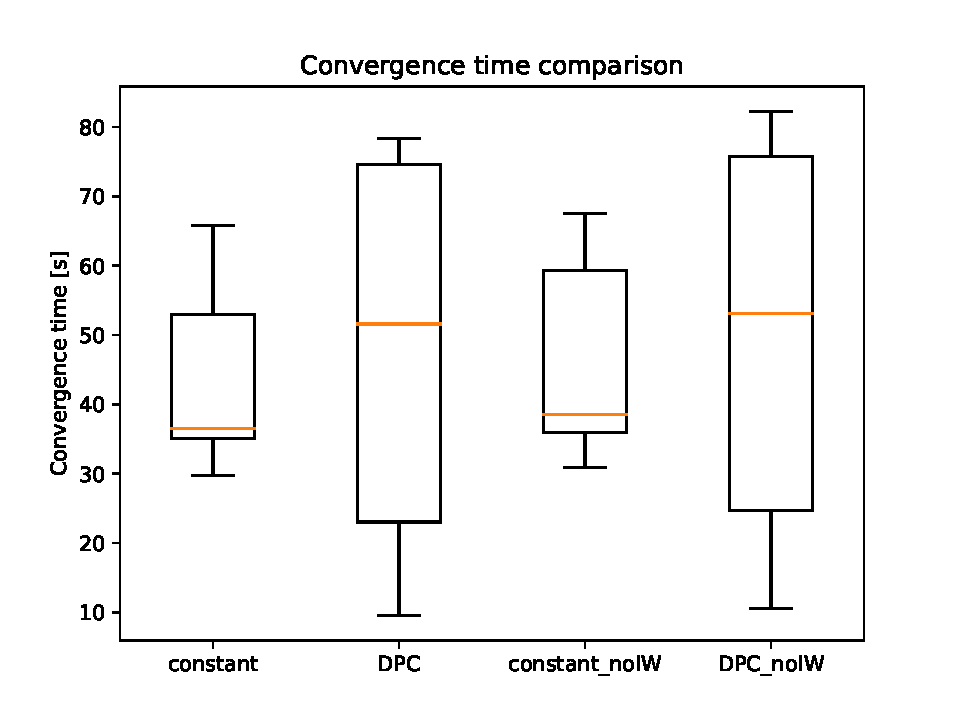
\includegraphics[width=\figwidth\columnwidth]{images/internet_like/dpc-vs-constant-30fixed/constant-dpc-comparison-30fixed_time_boxplot}
		\caption{Convergence time comparison between different environments}
		\label{fig:dpc_vs_constant_convergence_time}
		\qquad
	\end{subfigure}

	\begin{subfigure}{\columnwidth}
		\centering
		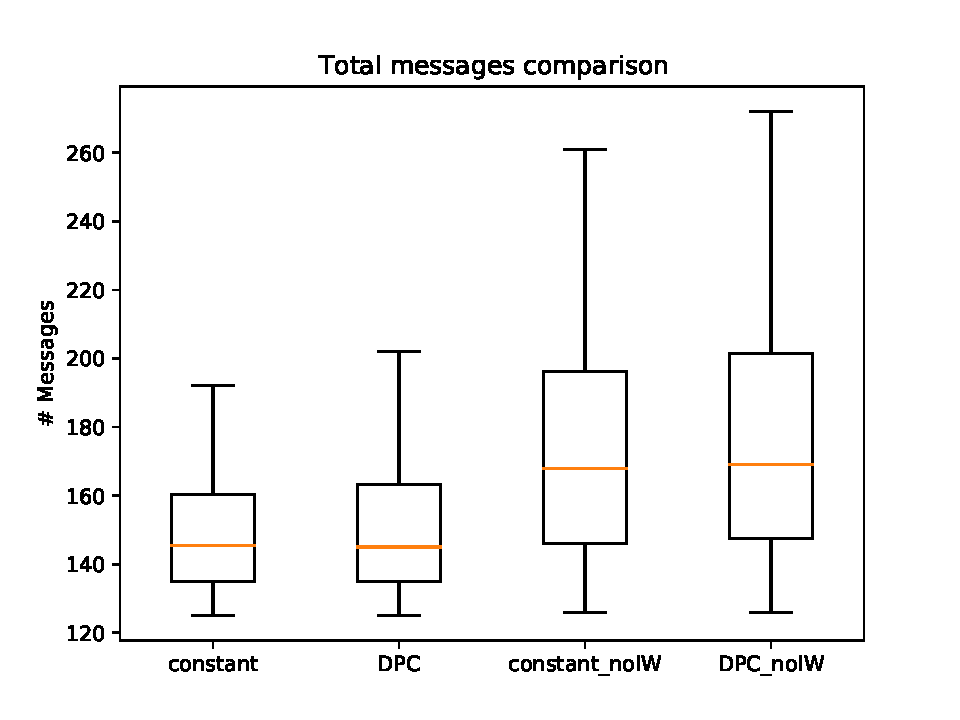
\includegraphics[width=\figwidth\columnwidth]{images/internet_like/dpc-vs-constant-30fixed/constant-dpc-comparison-30fixed_messages_boxplot}
		\caption{Messages necessary to reach the convergence comparison}
		\label{fig:dpc_vs_constant_messages}
		\qquad
	\end{subfigure}

	\caption{Comparison between the \ac{DPC} \ac{MRAI} strategy and the constant \ac{MRAI}
			 strategy, 100 experiments with the same conditions with $MRAI_{mean}$
			 equals to \num{30.0}}
	\label{fig:dpc_vs_constant}
	\vspace{\figvspace}
\end{figure}

So i decided to run the same experiments on an internet like topology of \num{1000}
nodes.
Always with $MRAI_{mean}$ of \num{30} and \num{100} different seeds.
The results are presented in \Cref{fig:dpc_vs_constant_1000}.

\begin{figure}[tb]
	\centering

	\begin{subfigure}{\columnwidth}
		\centering
		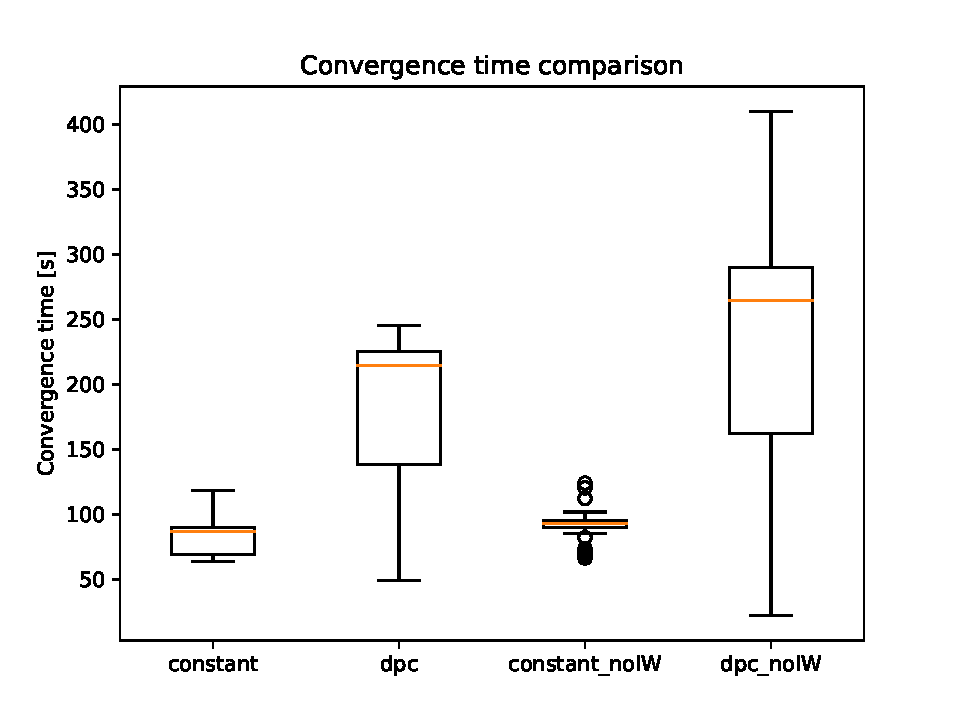
\includegraphics[width=\figwidth\columnwidth]{images/internet_like/dpc-vs-constant-30fixed/constant-dpc-1000-comparison-30fixed_time_boxplot.pdf}
		\caption{Convergence time comparison between different environments}
		\label{fig:dpc_vs_constant_convergence_time_1000}
		\qquad
	\end{subfigure}

	\begin{subfigure}{\columnwidth}
		\centering
		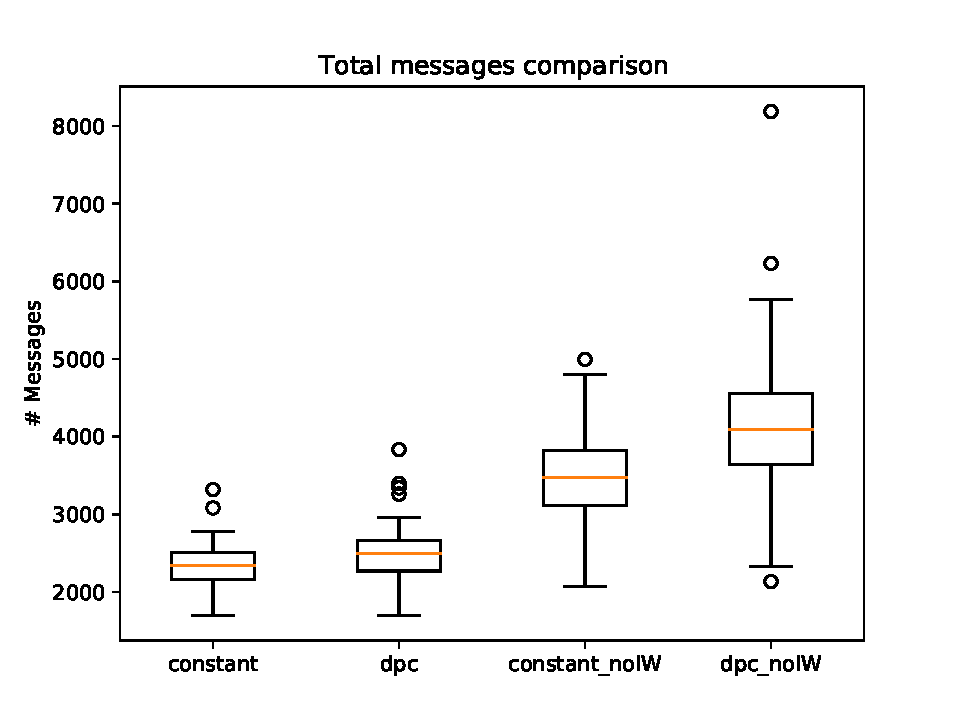
\includegraphics[width=\figwidth\columnwidth]{images/internet_like/dpc-vs-constant-30fixed/constant-dpc-1000-comparison-30fixed_messages_boxplot.pdf}
		\caption{Messages necessary to reach the convergence comparison}
		\label{fig:dpc_vs_constant_messages_1000}
		\qquad
	\end{subfigure}

	\caption{Comparison between the \ac{DPC} \ac{MRAI} strategy and the constant \ac{MRAI}
			 strategy, 100 experiments with the same conditions with $MRAI_{mean}$
			 equals to \num{30.0}, in an internet like graph with \num{1000} nodes}
	\label{fig:dpc_vs_constant_1000}
	\vspace{\figvspace}
\end{figure}

Some more general results could be saw taking into consideration the random \ac{MRAI}
strategy on the internet like graph.
The results are visible in \Cref{fig:random_mrai_pareto_freq}.
The first thing that we can see is that this time there are not huge spikes 
for certain messages amount.
The number of messages is more distributed between \num{145} and \num{152}, with 
some particulary dense columns.
Also, the convergence time is more distributed, thanks to the random \ac{MRAI} distribution.
We can guess that if a central node has a huge \ac{MRAI} timer and it transmits
incorrect information it would act as a bottleneck for the update with the 
correct information.

\begin{figure}[tb]
	\centering
	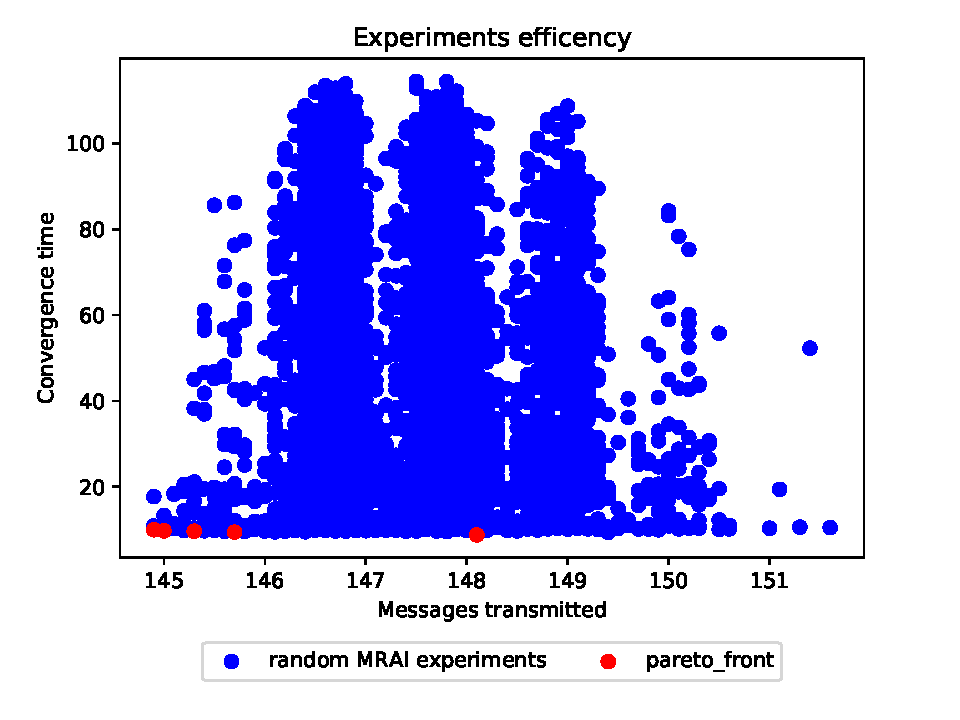
\includegraphics[width=\figwidth\columnwidth]{images/internet_like/graph-100-random/random-multiple_mrais}
	\caption{Pareto front in the Internet like random environment}
	\label{fig:random_mrai_pareto_freq}
	\vspace{\figvspace}
\end{figure}

From the comparison of the three \ac{MRAI} strategies we can see, in \Cref{fig:internet_pareto_comparison},
that the constant \ac{MRAI} covers a really small part of the random strategy,
and it has the tendency to produce a lot of messages for low $MRAI_{mean}$.
On the opposite side the \ac{DPC} strategy use more messages but the tendancy
is to keep the number of messages under a certain threshold.
And for small values of \ac{MRAI} is also possible for the constant strategy
to send more messages than the \ac{DPC} strategy.

\begin{figure}[tb]
	\centering
	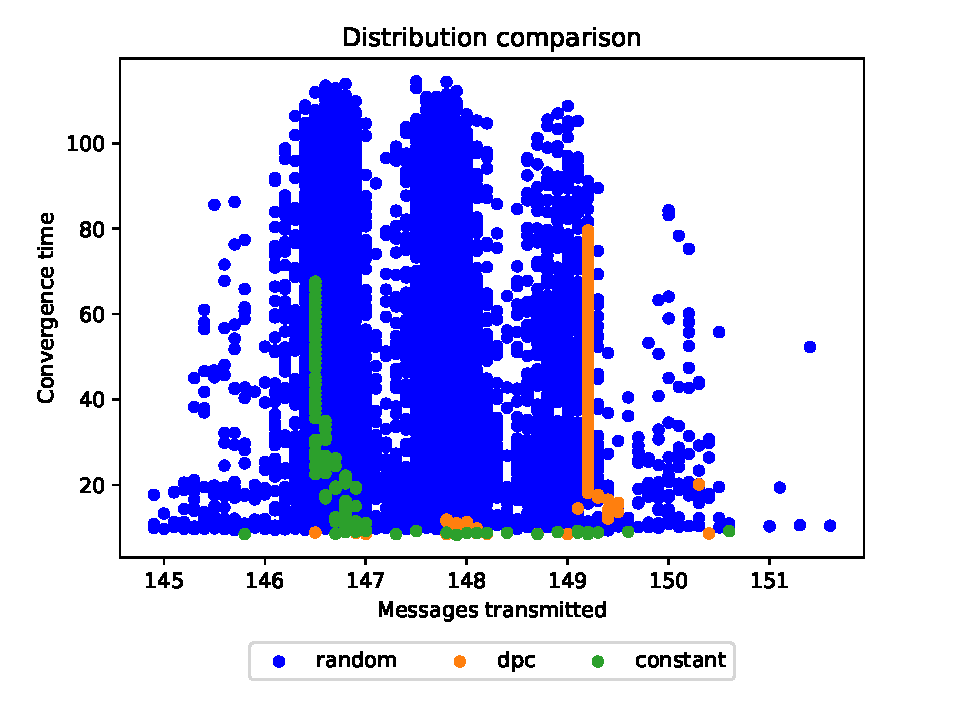
\includegraphics[width=\figwidth\columnwidth]{images/internet_like/internet_like_comparison}
	\caption{Comparison of the random strategy and the constant one in the internet like environment}
	\label{fig:internet_pareto_comparison}
	\vspace{\figvspace}
\end{figure}

I would like to study more deeply the first part of \Cref{fig:random_mrai_pareto_freq}.
In particular the experiments with convergence time lower than \num{20} and the
number of messages under \num{146}.
We would see what particular \ac{MRAI} settings those experiments has to produce
those good outputs.
The results are presented in \Cref{fig:random_study}.
In those plots we have on the $x$ axis the nodes ordered by centrality.
On the first $y$ axis we can see the load centrality value normalized.
The blue curve (that is equal on each plot, because the graph is one) represent
the centrality of each nodes, thanks to the fact that nodes are ordered by centrality
we see this line descending.
Is also noticable that the magiority of the nodes have a centrality of zero.
Each plot is divided in three sublplots that will help us to understand how \ac{MRAI}
is distributed in the graph.
The red line in the first subplot represent the out \ac{MRAI} mean of each node.
The out \ac{MRAI} of a node is the mean of the \ac{MRAI} setted on the output
links of the node.
The second plot contains the input \ac{MRAI} mean, that is the opposit of the
output \ac{MRAI} mean, so it's the mean of the \ac{MRAI}s used by the neighbors
with the node that we are analyzing.
The last subplot contains the absolute difference of the previous two lines.
Each point on those lines is the mean of all the graphs that produced results
in the reange of our interest.

We can clearly see a correlation between the \ac{MRAI} and the centrality.
It would become even clearer using the second plot that contains also the sandard
variation between all the means of the graphs in \Cref{fig:random_study_std}.

\begin{figure}[tb]
	\centering

	\begin{subfigure}{\columnwidth}
		\centering
		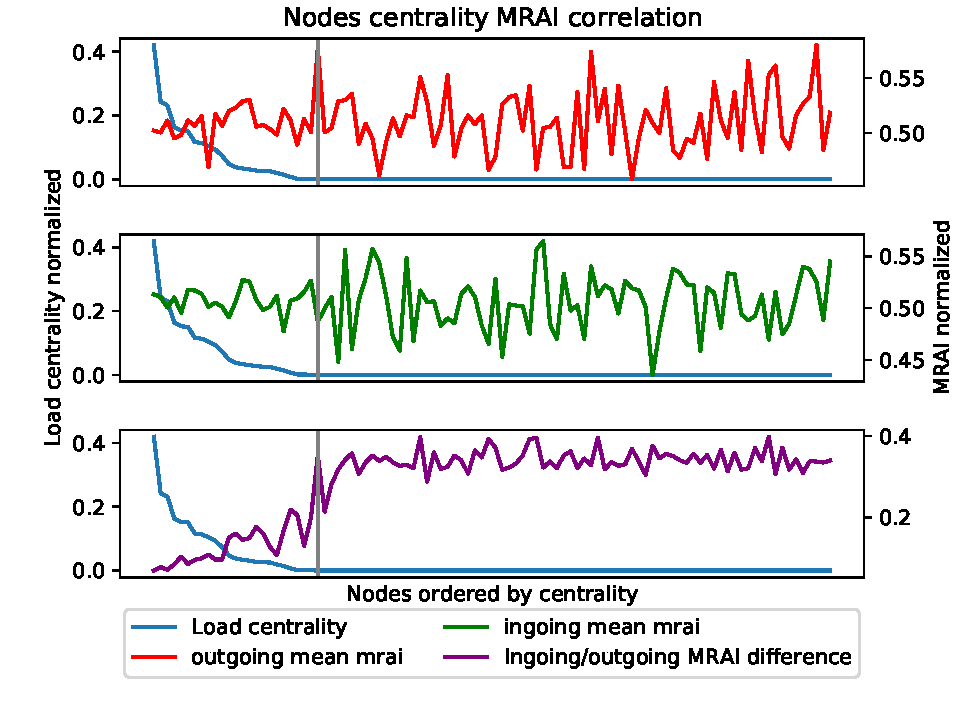
\includegraphics[width=\figwidth\columnwidth]{images/internet_like/graph-100-random/random_study}
		\caption{Study of the best results in the random experiments}
		\label{fig:random_study_lines}
		\qquad
	\end{subfigure}

	\begin{subfigure}{\columnwidth}
		\centering
		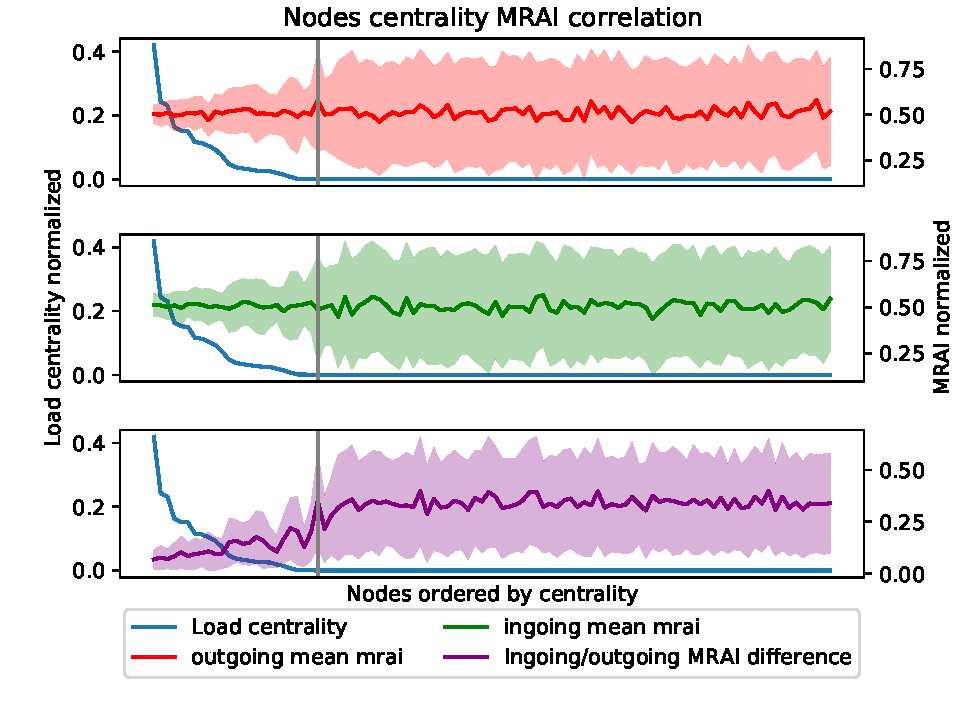
\includegraphics[width=\figwidth\columnwidth]{images/internet_like/graph-100-random/random_study_std}
		\caption{Study of the best result in the random experiments showing the standard deviation}
		\label{fig:random_study_std}
		\qquad
	\end{subfigure}

	\caption{Best random experiments, on the internet like topology, shows the 
			 correlation between centrality and the \ac{MRAI} of the nodes, the
			 gray wertical line represent the first node with centrality of 0}
	\label{fig:random_study}
	\vspace{\figvspace}
\end{figure}


\bibliographystyle{IEEEtran}
\bibliography{references}

\end{document}
